\documentclass[a4paper,titlepage,12pt]{report}	%El modo de documento es para la numeración.

\usepackage{graphicx} %Imágenes
\usepackage[utf8]{inputenc} %Tildes
\usepackage[spanish,es-tabla]{babel} %Español, es-table: llamar tablas en vez de cuadros
\usepackage[breaklinks=true]{hyperref} %Hiperenlaces
\usepackage{amssymb, amsmath, amsbsy} %Símbolos matemáticos
\usepackage{float} %Mover las imágenes usando [H]
\usepackage{eurosym} %Símbolo de euro \euro
\usepackage{listings} %Código
\usepackage{listingsutf8} %Tildes en listings

\numberwithin{figure}{section} %Hace que la primera figura de cada sección X sea X.1
\numberwithin{table}{section} %Hace que la primera tabla de cada sección X sea X.1

\begin{document}
	\lstset{inputencoding=utf8/latin1} %Tildes en listlings
	\begin{titlepage}
		\begin{center}
			\begin{figure}[htb]
				\begin{center}
					
\includegraphics[width=12cm]{./Portada/ugr.png}
				\end{center}
			\end{figure}

			\vspace*{0.8cm}
			\begin{Large}
				\textbf{Grado en Ingeniería Informática.}\\
			\end{Large}
			\begin{Huge}
				\vspace{1.5cm}
				\textbf{Cuestiones opcionales.} \\
			\end{Huge}
			\vspace*{0.76cm}
			\rule{100mm}{0.1mm}\\
			\vspace*{0.5cm}
			\begin{large}
				\textbf{Nombre de la asignatura:}\\
				Ingeniería de Servidores.\\
				\vspace*{0.5cm}
				\textbf{Realizado por:}\\
				Néstor Rodríguez Vico \\

				\vspace*{2cm}
				\begin{figure}[htb]
					\begin{center}
						
\includegraphics[width=5cm]{./Portada/etsiit.png}
					\end{center}
				\end{figure}
				\vspace*{-0.6cm}
				ESCUELA TÉCNICA SUPERIOR DE INGENIERÍAS INFORMÁTICA Y DE TELECOMUNICACIÓN.\\
				\rule{20mm}{0.1mm}\\
				\vspace*{0.6cm}
				Granada, \today.
			\end{large}
		\end{center}
	\end{titlepage}

	%--------------Indices--------------
	\tableofcontents
	\clearpage
	\listoffigures %Imagenes
	\clearpage
	%----------------------------------

	\chapter[Práctica 1.]{Práctica 1.}

	\section[Cuestión opcional 1: Muestre (con capturas de pantalla) cómo ha comprobado que el RAID1 funciona.]{Cuestión opcional 1: Muestre (con capturas de pantalla) cómo ha comprobado que el RAID1 funciona.}

	Para probar que funciona correctamente vamos a hacer una simulación de fallo y a arreglar el daño causado para ver si el disco se sincroniza correctamente. El proceso es el que sigue: \cite{comprobarRAID} \\

	Primero vamos a simular un fallo software. Para ello usamos el comando \textit{sudo mdadm --manage --set-faulty /dev/md0 /dev/sdb1} como se muestra en la figura \ref{P1-comprobacionRAID1}.

	\begin{figure}[H]
		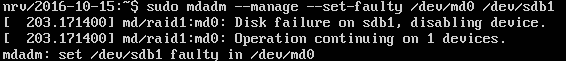
\includegraphics[width=\linewidth]{./Imagenes/P1/ComprobarRAID1.png}
		\vspace{-0.5cm}
		\caption[Simulación fallo software.]{Simulación fallo software.}
		\label{P1-comprobacionRAID1}
	\end{figure}

	Para ver que correctamente se ha producido el fallo veremos el estado del disco. Para ello usamos el comando \textit{sudo mdadm --detail /dev/md0} como se muestra en la figura \ref{P1-comprobacionRAID2}.

	\begin{figure}[H]
		\centering
		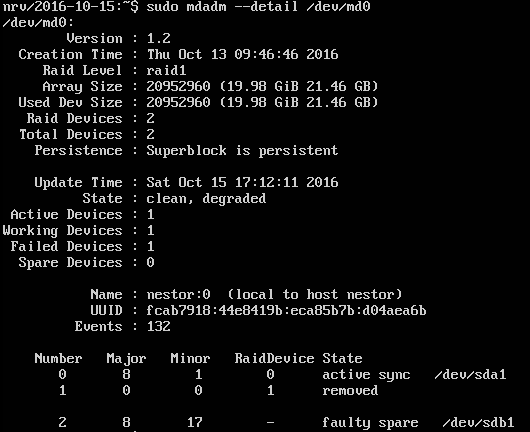
\includegraphics[scale=0.68]{./Imagenes/P1/ComprobarRAID2.png}
		\caption[Comprobación del fallo software.]{Comprobación del fallo software.}
		\label{P1-comprobacionRAID2}
	\end{figure}

	Para arreglar el fallo producido vamos a retirar en caliente el disco. Para ello usamos el comando \textit{sudo mdadm /dev/md0 -r /dev/sdb1} como se muestra en la figura \ref{P1-comprobacionRAID3}.

	\begin{figure}[H]
		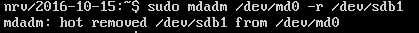
\includegraphics[width=\linewidth]{./Imagenes/P1/ComprobarRAID3.png}
		\vspace{-0.5cm}
		\caption[Retirada en caliente del disco.]{Retirada en caliente del disco.}
		\label{P1-comprobacionRAID3}
	\end{figure}

	Para finalizar, volvemos a añadir el disco. Para ello usamos el comando \textit{sudo mdadm /dev/md0 -a /dev/sdb1} como se muestra en la figura \ref{P1-comprobacionRAID4}.

	\begin{figure}[H]
		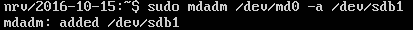
\includegraphics[width=\linewidth]{./Imagenes/P1/ComprobarRAID4.png}
		\vspace{-0.5cm}
		\caption[Añadir el disco a \textit{/dev/sdb1}.]{Añadir el disco a \textit{/dev/sdb1}.}
		\label{P1-comprobacionRAID4}
	\end{figure}

	Para ver que todo ha ido correctamente sólo tenemos que comprobar el estado del disco. Para ello usamos el comando \textit{sudo mdadm --detail /dev/md0} como se muestra en la figura \ref{P1-comprobacionRAID5}.

	\begin{figure}[H]
		\centering
		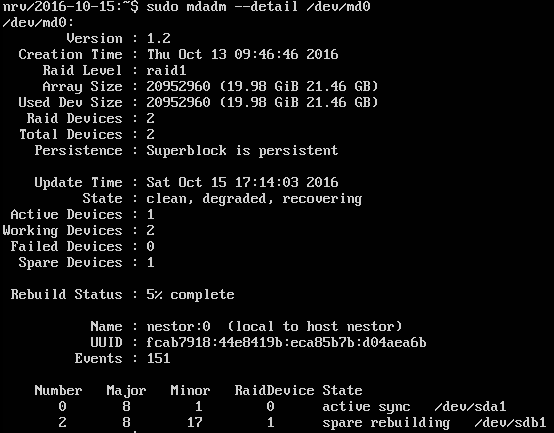
\includegraphics[scale=0.73]{./Imagenes/P1/ComprobarRAID5.png}
		\caption[Comprobación final.]{Comprobación final.}
		\label{P1-comprobacionRAID5}
	\end{figure}

	\section[Cuestión opcional 2: ¿Qué relación hay entre los atajos de teclado de emacs y los de la consola bash? ¿y entre los de vi y las páginas del manual?]{Cuestión opcional 2: ¿Qué relación hay entre los atajos de teclado de emacs y los de la consola bash? ¿y entre los de vi y las páginas del manual?}

	La relación se debe a que el \textit{bash} se puede poner en varios modos, y uno de ellos es el modo \textit{emacs}. \cite{bashemacs}

	La relación es que en ambos se usan los mismos comando. Para ver los comandos que se usan en \textit{man} podemos ejecutar \textit{man man} y a continuación pulsar \textit{h} para ver los diferentes comandos. Los comandos de \textit{vi} podemos verlos en la página de IBM \cite{vi}. Por ejemplo, para ir a la última línea de la página en ambos casos debemos pulsar la tecla \textit{G}.

	\chapter[Práctica 2.]{Práctica 2.}

	%%%%%%%%%%%%%%%%%%%%%%%%%%%%%%%%%%%%%%%%%%%%%%%%%%%%
	%%%%%%%%%%%%%%%%%%%% Cuestión Opcional 1 %%%%%%%%%%%
	%%%%%%%%%%%%%%%%%%%%%%%%%%%%%%%%%%%%%%%%%%%%%%%%%%%%
	\section[Cuestión opcional 1: Instale y pruebe terminator y/o tmux. Con screen, pruebe su funcionamiento dejando sesiones ssh abiertas en el servidor y recuperándolas posteriormente.]{Cuestión opcional 1: Instale y pruebe terminator y/o tmux. Con screen, pruebe su funcionamiento dejando sesiones ssh abiertas en el servidor y recuperándolas posteriormente.}

	Para instalar \textit{terminator} debemos ejecutar \textit{sudo apt install terminator}. Para instalar \textit{screen} debemos ejecutar \textit{sudo apt install screen}. Aprender a usar \textit{terminator}, a un nivel suficiente para la realización de este ejercicio, es fácil. Pero para aprender a usar \textit{screen} he consultado las páginas del manual \cite{screen}. \\

	\begin{enumerate}
		\item Lo primero que he hecho ha sido crear tres terminales en \textit{terminator}, dos para usar \textit{screen} y realizar dos conexiones ssh a mi servidor y una tercera para comprobar el estado de las dos anteriores. En las dos terminales superiores que se ven en la figura \ref{P2-O1-1} he abierto dos sesiones de \textit{screen}. Para ello he ejecutado \textit{screen -S ssh1} en la terminal de la izquierda y \textit{screen -S ssh2} en la terminal de la derecha. Para corroborar que estamos en \textit{screen}, he ejecutado en ambas \textit{echo \$TERM} y efectivamente podemos ver que estamos en screen mientras que en la terminal inferior no. También podemos ver en la terminal inferior como hay dos sesiones de \textit{screen} abiertas. En las terminales superiores he realizado dos conexiones ssh, y he ejecutado dos comandos para ver que, efectivamente, funcionan. Todo este proceso se puede ver en la igura \ref{P2-O1-1}.
		\item A continuación, cerramos \textit{terminator}. Lo abrimos de nuevo y creamos las mismas tres terminales. Podemos comprobar que no estamos en una sesión de \textit{screen} ejecutando \textit{echo \$TERM} y vemos que no estamos en una sesión de \textit{screen}. Para restaurar las sesiones, ejecutamos \textit{screen -r 9417.ssh2} y \textit{screen -r 9403.ssh1}, como podemos ver en la figura \ref{P2-O1-2}.
		\item Tras ejecutar los dos comandos anteriores, podemos ver que se restauran las sesiones de \textit{screen} y las conexiones ssh. Una vez más ejecutamos \textit{echo \$TERM} para ver que, correctamente, estamos en las sesiones de \textit{screen}. Todo este proceso lo podemos ver en la figura \ref{P2-O1-3}.
		\item Para cerrar la sesión de \textit{screen} ejecutamos \textit{exit} dos veces, la primera de ellas para cerrar la conexión ssh y la segunda para cerrar la conexión de \textit{screen}. Finalmente, ejecutamos de nuevo \textit{echo \$TERM} para ver que no estamos en una sesión de \textit{screen}. En la terminal inferior ejecutamos \textit{screen -ls} para ver que no queda ninguna sesión de \textit{screen} abierta. Todo lo comentado podemos verlo en la figura \ref{P2-O1-4}.
	\end{enumerate}

	\begin{figure}[H]
		\centering
		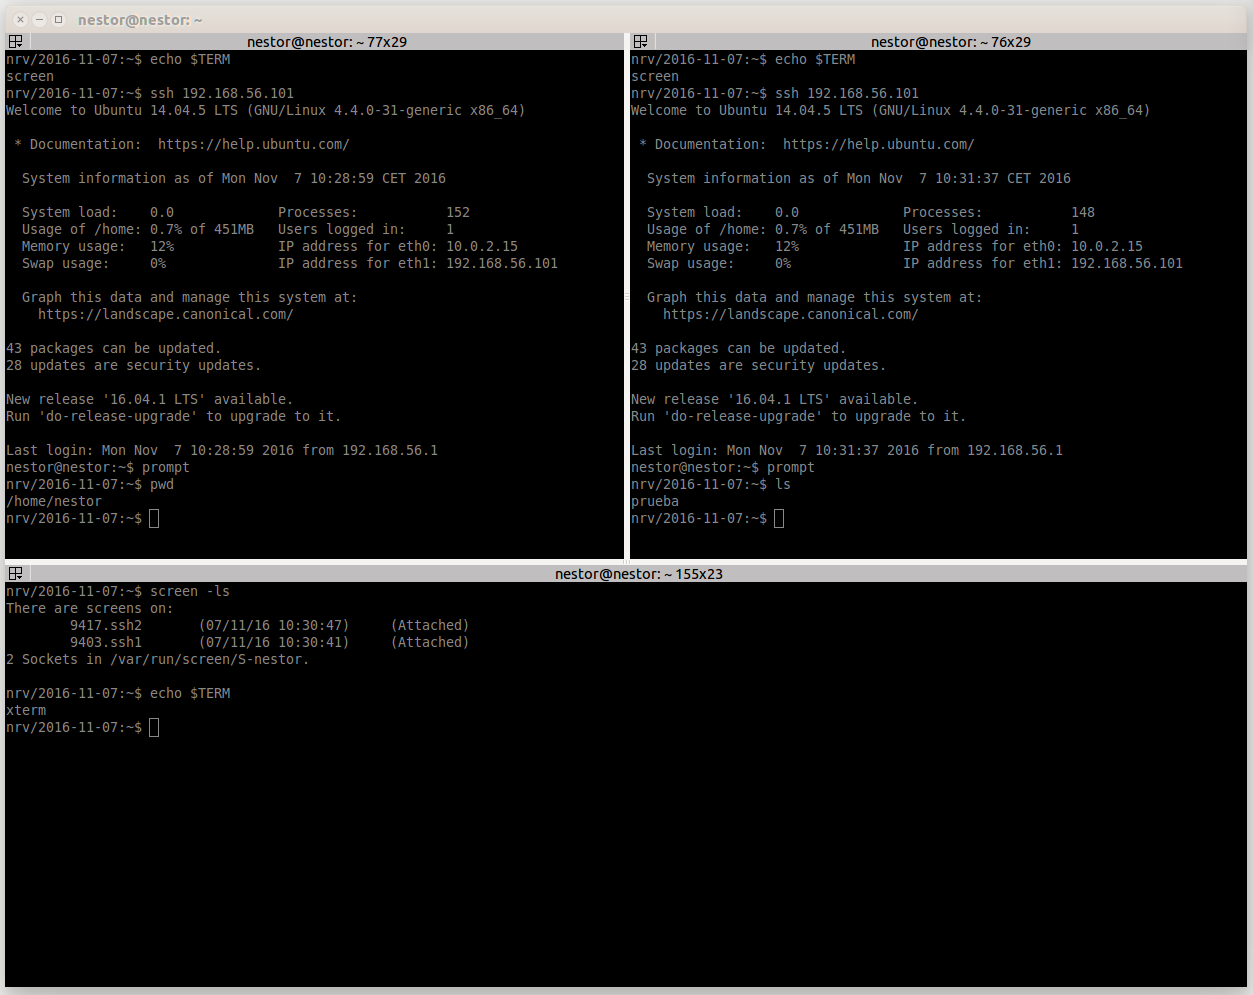
\includegraphics[scale=0.29]{./Imagenes/P2/O1-1.png}
		\caption[Creación de las sesiones de \textit{screen}.]{Creación de las sesiones de \textit{screen}.}
		\label{P2-O1-1}
	\end{figure}

	\begin{figure}[H]
		\centering
		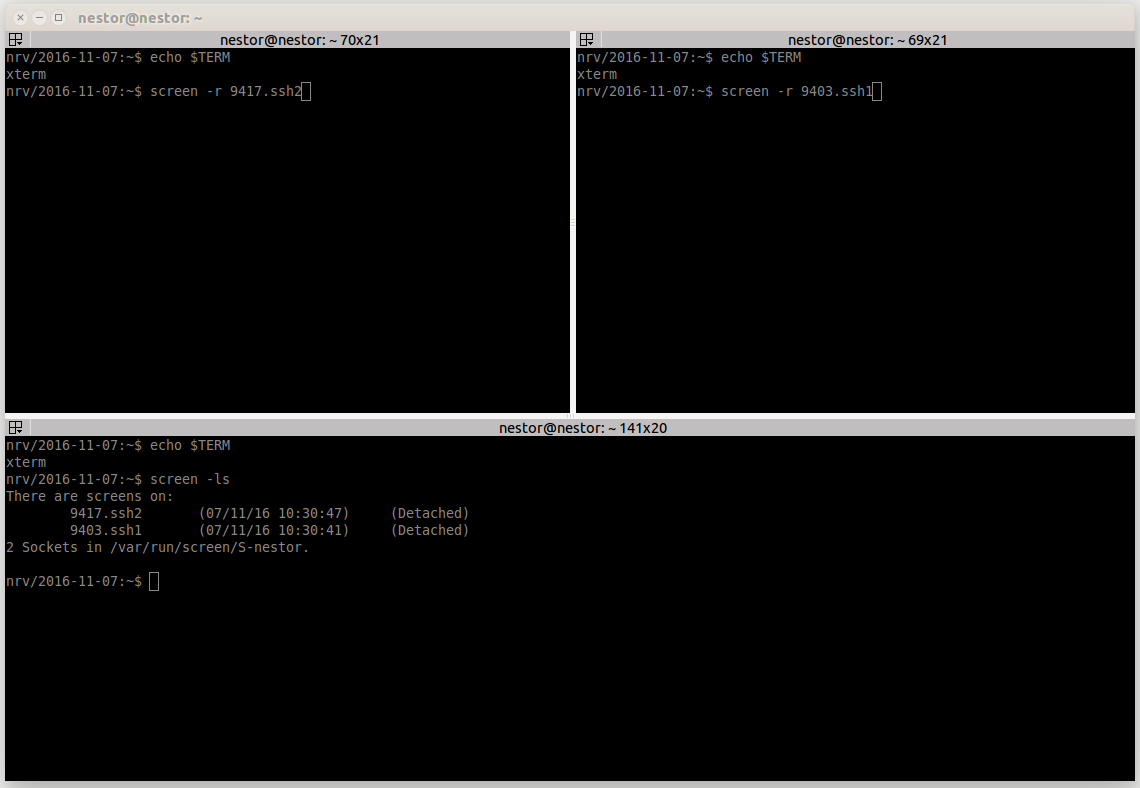
\includegraphics[scale=0.32]{./Imagenes/P2/O1-2.png}
		\caption[Restauración de las sesiones de \textit{screen}.]{Restauración de las sesiones de \textit{screen}.}
		\label{P2-O1-2}
	\end{figure}

	\begin{figure}[H]
		\centering
		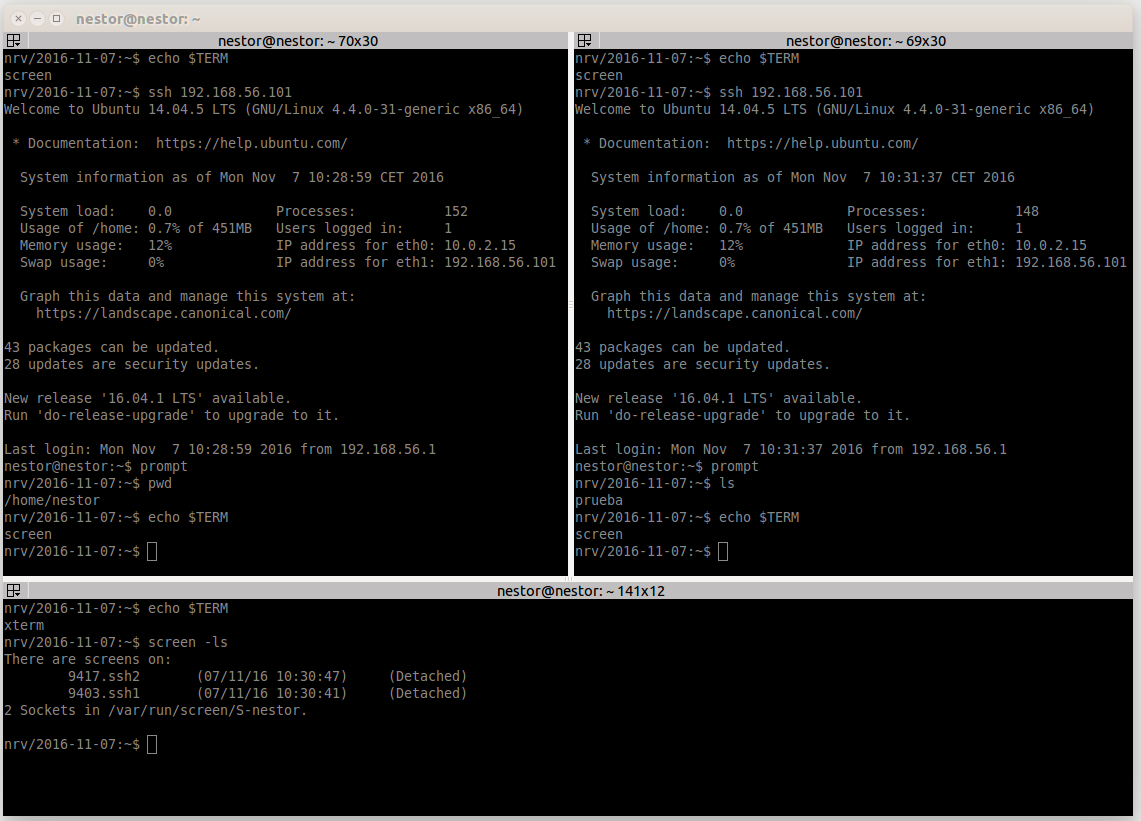
\includegraphics[scale=0.31]{./Imagenes/P2/O1-3.png}
		\caption[Sesiones de \textit{screen} restauradas.]{Sesiones de \textit{screen} restauradas.}
		\label{P2-O1-3}
	\end{figure}

	\begin{figure}[H]
		\centering
		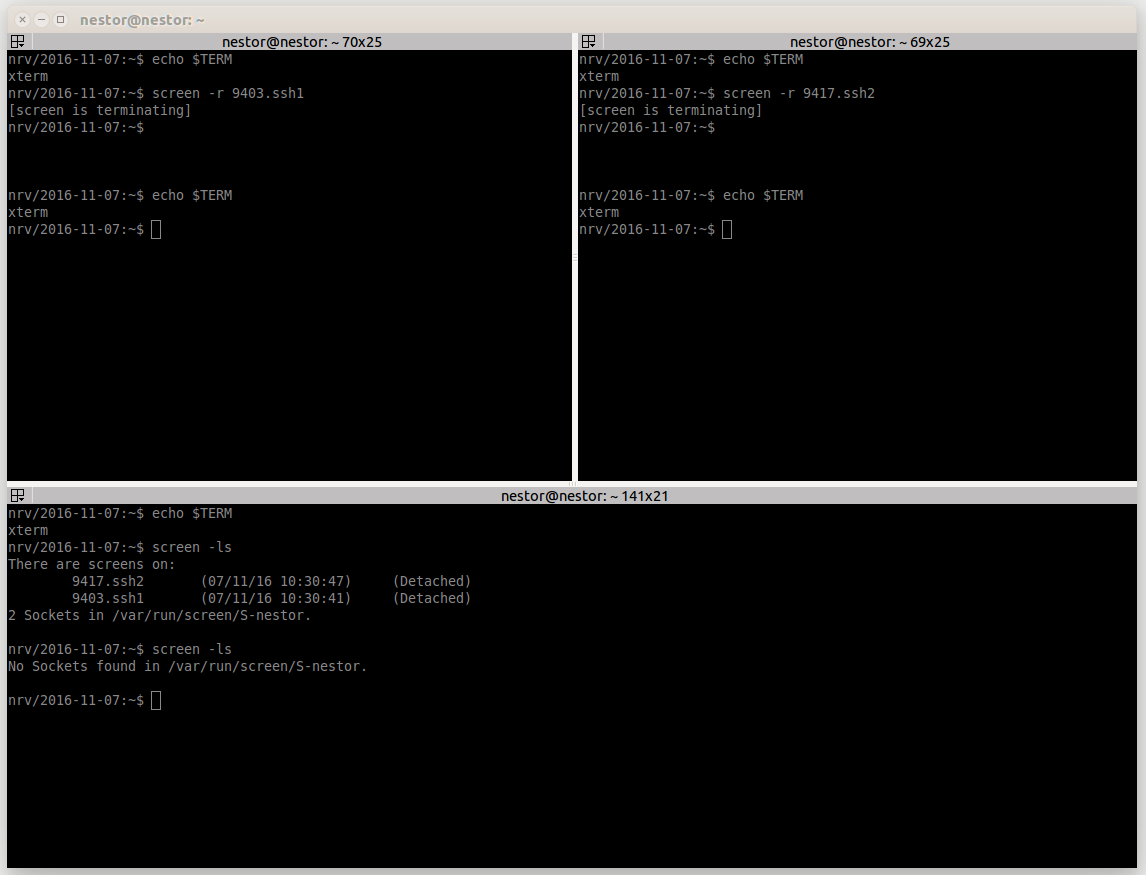
\includegraphics[scale=0.31]{./Imagenes/P2/O1-4.png}
		\caption[Sesiones de \textit{screen} cerradas.]{Sesiones de \textit{screen} cerradas.}
		\label{P2-O1-4}
	\end{figure}

	%%%%%%%%%%%%%%%%%%%%%%%%%%%%%%%%%%%%%%%%%%%%%%%%%%%%
	%%%%%%%%%%%%%%%%%%%% Cuestión Opcional 2 %%%%%%%%%%%
	%%%%%%%%%%%%%%%%%%%%%%%%%%%%%%%%%%%%%%%%%%%%%%%%%%%%
	\section[Cuestión opcional 2: Instale el servicio y pruebe su funcionamiento.]{Cuestión opcional 2: Instale el servicio y pruebe su funcionamiento.}

	Para ver el funcionamiento de \textit{fail2ban} podemos visitar la página oficial de dicho servicio \cite{fail2ban}. Como página complementaria voy a usar Digital Ocean \cite{fail2bandigitalocean}. Para instalar \textit{fail2ban} debemos ejecutar el comando \textit{sudo apt install fail2ban}. Una vez instalado, lo recomendable es copiar el archivo \textit{/etc/fail2ban/jail.conf} para evitar problemas en futuras actualizaciones. Para ello, ejecutamos el comando \textit{sudo cp /etc/fail2ban/jail.conf /etc/fail2ban/jail.local}, como podemos ver en la figura \ref{P2-O2-copiarjail}.
	\begin{figure}[H]
		\centering
		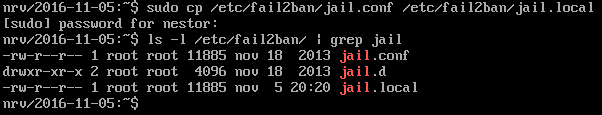
\includegraphics[scale=0.53]{./Imagenes/P2/O2-copiarjail.png}
		\caption[Copia del archivo \textit{/etc/fail2ban/jail.conf}.]{Copia del archivo \textit{/etc/fail2ban/jail.conf}.}
		\label{P2-O2-copiarjail}
	\end{figure}

	Para ver su funcionamiento, voy a intentar conectarme a mi servidor \textit{ssh} pero fallaré la contraseña para ver que \textit{fail2ban} funciona correctamente. Como en mi máquina anfitriona tengo configurado \textit{ssh} para permitir el acceso sin contraseña, voy a realizar el intento de acceso desde CentOS, como podemos ver en la figura \ref{P2-O2-accesomal}.
	\begin{figure}[H]
		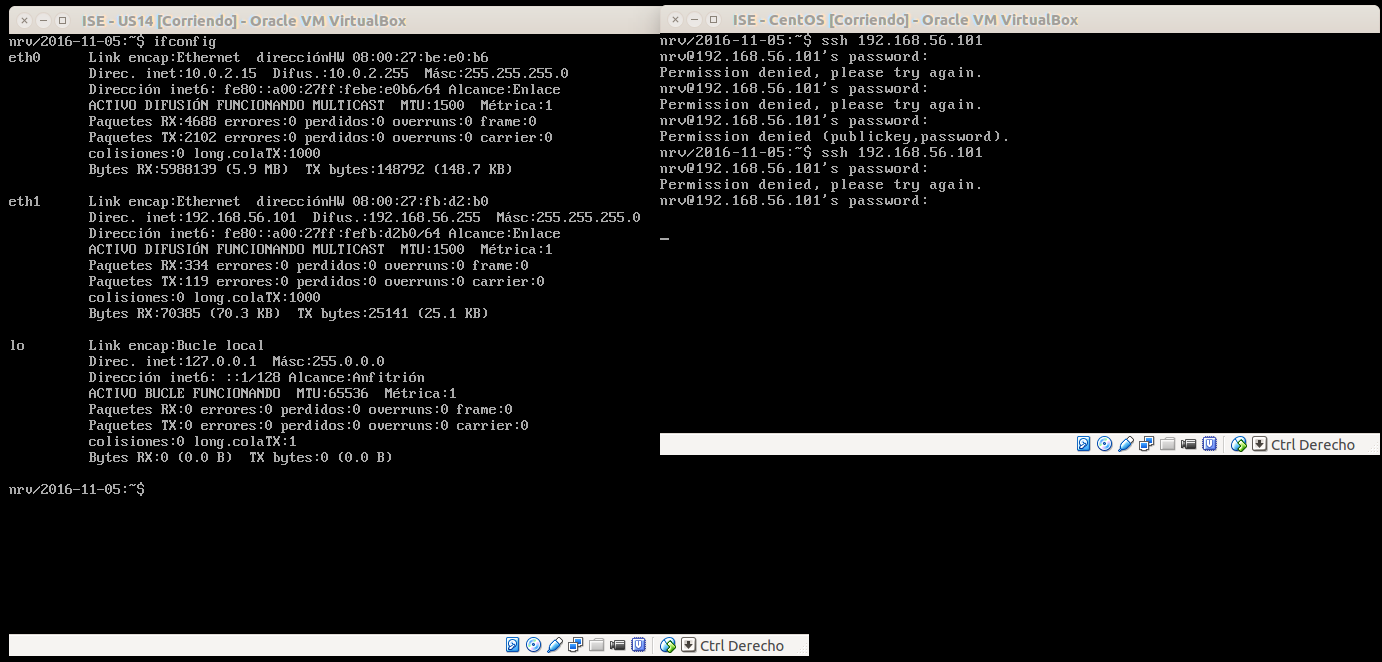
\includegraphics[width=\linewidth]{./Imagenes/P2/O2-accesomal.png}
		\vspace{-0.5cm}
		\caption[Acceso incorrecto (máquinas conectadas en modo \textit{host-only}).]{Acceso incorrecto (máquinas conectadas en modo \textit{host-only}).}
		\label{P2-O2-accesomal}
	\end{figure}

	Desde nuestro servidor, ejecutando el comando \textit{sudo iptables -S} vemos que se ha bloqueado la conexión ssh para la IP \textit{} que es la IP de mi máquina virtual de CentOS, como podemos ver en la figura \ref{P2-O2-iptables}.
	\begin{figure}[H]
		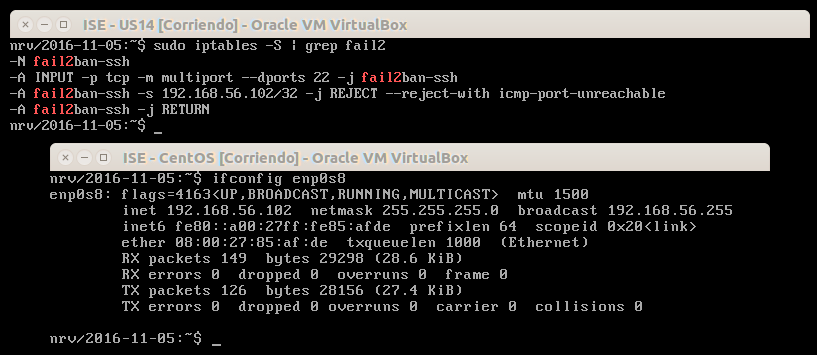
\includegraphics[width=\linewidth]{./Imagenes/P2/O2-iptables.png}
		\vspace{-0.5cm}
		\caption[Dirección IP bloqueada (máquinas conectadas en modo \textit{\textbf{bridge}}).]{Dirección IP bloqueada (máquinas conectadas en modo \textit{\textbf{bridge}}).}
		\label{P2-O2-iptables}
	\end{figure}

	%%%%%%%%%%%%%%%%%%%%%%%%%%%%%%%%%%%%%%%%%%%%%%%%%%%%
	%%%%%%%%%%%%%%%%%%%% Cuestión Opcional 3 %%%%%%%%%%%
	%%%%%%%%%%%%%%%%%%%%%%%%%%%%%%%%%%%%%%%%%%%%%%%%%%%%
	\section[Cuestión opcional 3: Instale el servicio y pruebe su funcionamiento.]{Cuestión opcional 3: Instale el servicio y pruebe su funcionamiento.}

	Para ver el funcionamiento de \textit{rkhunter} podemos visitar la página oficial de dicho servicio \cite{rkhunter}. Para instalar el servicio ejecutamos \textit{sudo apt install rkhunter}. Lo primero que hacemos es crear una base de datos de como se encuentra nuestro sistema en el momento actual, para luego usarla como refeP2-rencia. Para ello ejecutamos el comando \textit{sudo rkhunter {-}-propupd}, como podemos ver en la figura \ref{P2-O3-propupd}.
	\begin{figure}[H]
		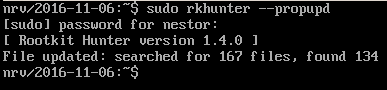
\includegraphics[width=\linewidth]{./Imagenes/P2/O3-propupd.png}
		\vspace{-0.5cm}
		\caption[Creación de la base de datos para \textit{rkhunter}.]{Creación de la base de datos para \textit{rkhunter}.}
		\label{P2-O3-propupd}
	\end{figure}

	Una vez hemos creado la base de datos, podemos analizar nuestro sistema ejecutando \textit{sudo rkhunter -c {-}-enable all}. Una vez acabado el análisis, podemos ver un resumen del análisis, como podemos ver en la figura \ref{P2-O3-analisis}.
	\begin{figure}[H]
		\centering
		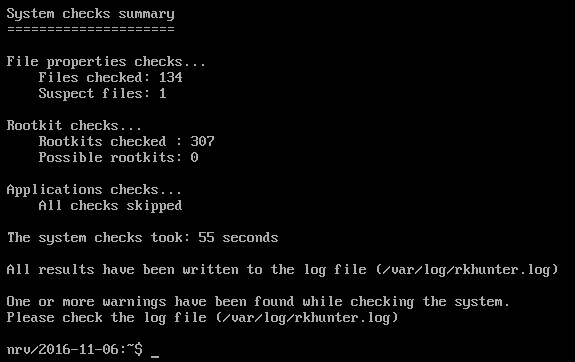
\includegraphics[scale=0.75]{./Imagenes/P2/O3-analisis.png}
		\caption[Resultado del análisis del sistema con \textit{rkhunter}.]{Resultado del análisis del sistema con \textit{rkhunter}.}
		\label{P2-O3-analisis}
	\end{figure}

	Como podemos ver en la figura \ref{P2-O3-analisis}, si queremos ver el resultado completo debemos ver el contenido del archivo \textit{/var/log/rkhunter.log}. Finalmente, si queremos actualizar la base de datos que creamos anteriormente, debemos ejecutar el comando \textit{sudo rkhunter {-}-update}

	%%%%%%%%%%%%%%%%%%%%%%%%%%%%%%%%%%%%%%%%%%%%%%%%%%%%
	%%%%%%%%%%%%%%%%%%%% Cuestión Opcional 4 %%%%%%%%%%%
	%%%%%%%%%%%%%%%%%%%%%%%%%%%%%%%%%%%%%%%%%%%%%%%%%%%%
	\section[Cuestión opcional 4: Realice la instalación de uno de estos dos “web containers” y pruebe su ejecución.]{Cuestión opcional 4: Realice la instalación de uno de estos dos “web containers” y pruebe su ejecución.}

	Voy a probar Apache Tomcat \cite{apachetomcat} en Ubuntu Server. Para instalar Apache Tomat, primero debemos ver si tenemos instalado Java instalado. Para ello, ejecutamos el comando \textit{java -version}. Como podemos ver en la figura \ref{P2-O4-javaversion} Java no se encuentra instalado, para instalarlo ejecutamos \textit{sudo apt-get install default-jdk}
	\begin{figure}[H]
		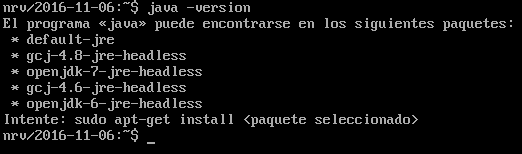
\includegraphics[width=\linewidth]{./Imagenes/P2/O4-javaversion.png}
		\vspace{-0.5cm}
		\caption[Java no se encuentra instalado de Ubuntu Server.]{Java no se encuentra instalado de Ubuntu Server.}
		\label{P2-O4-javaversion}
	\end{figure}

	Una vez hemos instalado java, ejecutamos \textit{sudo apt install tomcat7} para instalar Apache Tomcat. Para ver su funcionamiento, desde la máquina anfitriona vamos a un navegador y escribimos la dirección IP de nuestro servido web seguido de \textit{:8080}. En mi caso, como podemos ver en la figura \ref{P2-O4-ip}, la dirección IP de mi servidos es \textit{192.168.56.101}, por lo tanto en el navegador debemos ir a la dirección \textit{192.168.56.101:8080}. Como podemos ver en la figura \ref{P2-O4-tomcat}, el servicio funciona correctamente.
	\begin{figure}[H]
		\centering
		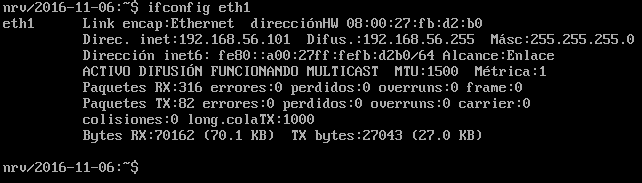
\includegraphics[scale=0.6]{./Imagenes/P2/O4-ip.png}
		\caption[Dirección IP de mi servidor.]{Dirección IP de mi servidor.}
		\label{P2-O4-ip}
	\end{figure}

	\begin{figure}[H]
		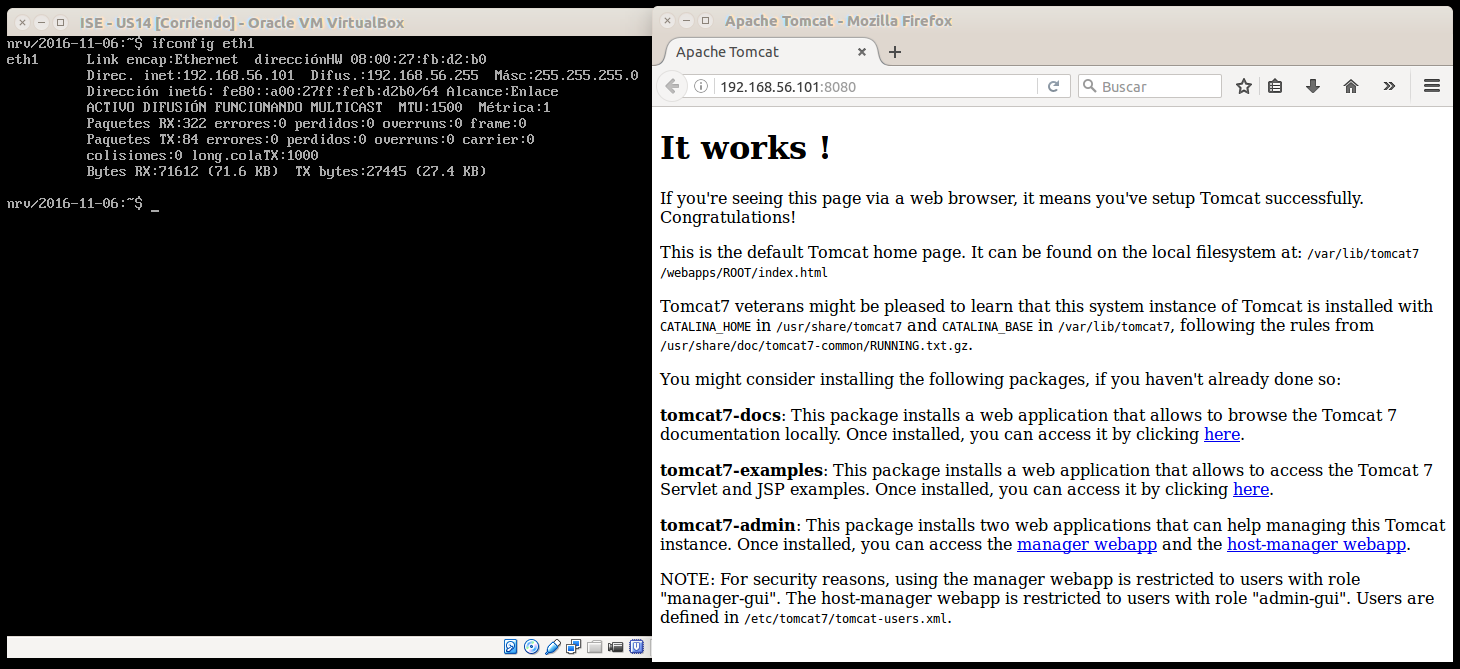
\includegraphics[width=\linewidth]{./Imagenes/P2/O4-tomcat.png}
		\vspace{-0.5cm}
		\caption[Servicio \textit{tomcat} funcionando correctamente (máquinas conectadas en modo \textit{host-only}).]{Servicio \textit{tomcat} funcionando correctamente (máquinas conectadas en modo \textit{host-only}).}
		\label{P2-O4-tomcat}
	\end{figure}

	Para acceder al gestor de aplicaciones, como podemos ver en la página de Apache Tomcat \cite{apachetomcatmanager} debemos acceder a la dirección \textit{192.168.56.101:8080/manager/html}. Una vez en esa dirección, nos pide un usuario y una contraseña. Para acceder he creado un usuario con los roles que se puede ver en la figura \ref{P2-O4-tomcat2} y he accedido con el. Dentro de tomcat podemos ver que se puede gestionar diferentes parámetros, como puede ser el tiempo que tardará en expirar una sesión inactiva, como se puede ver en la figura \ref{P2-O4-tomcat2}.

	\begin{figure}[H]
		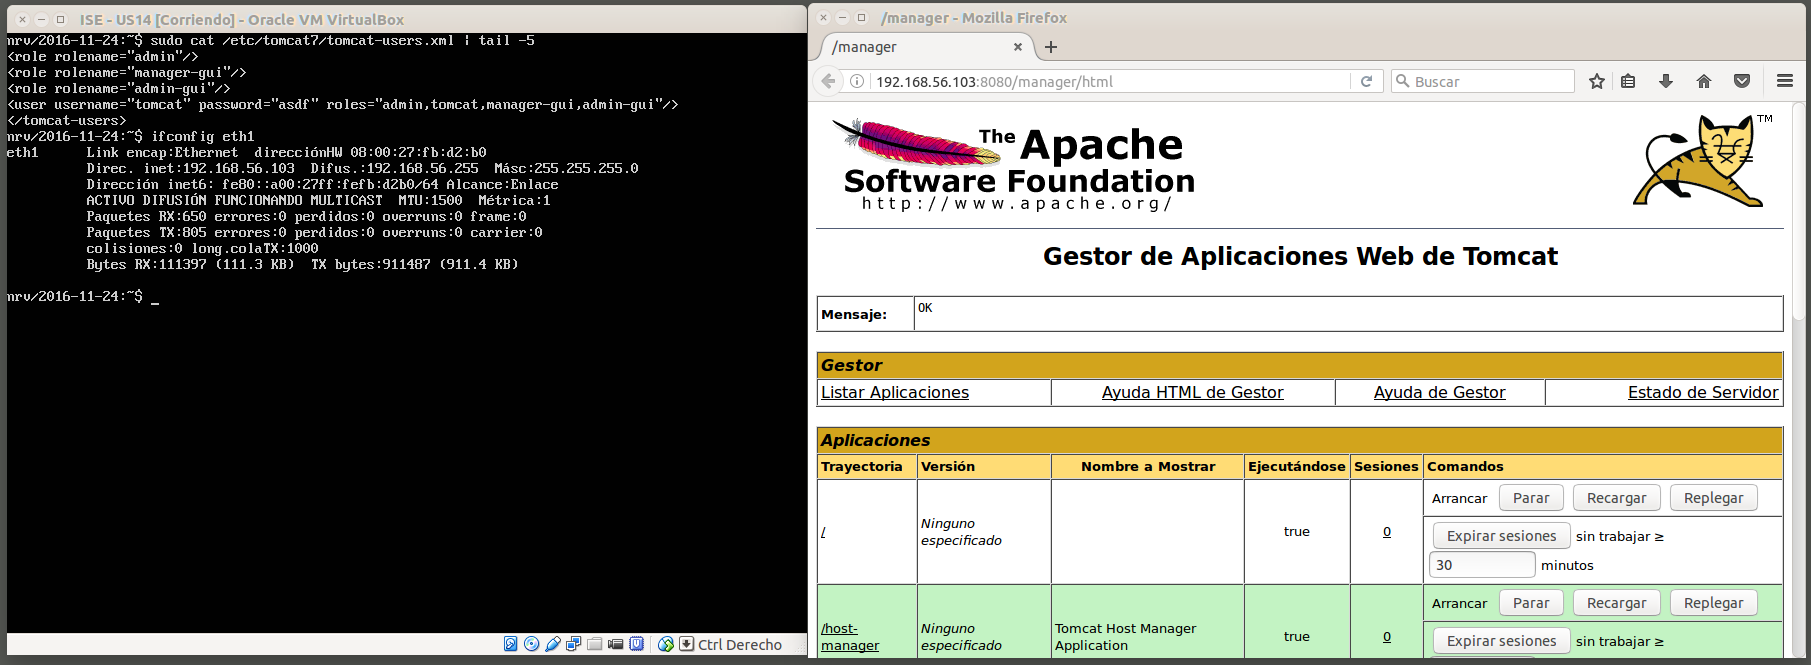
\includegraphics[width=\linewidth]{./Imagenes/P2/O4-tomcat2.png}
		\vspace{-0.5cm}
		\caption[Sesión iniciada en \textit{tomcat} (máquinas conectadas en modo \textit{host-only}).]{Sesión iniciada en \textit{tomcat} (máquinas conectadas en modo \textit{host-only}).}
		\label{P2-O4-tomcat2}
	\end{figure}

	%%%%%%%%%%%%%%%%%%%%%%%%%%%%%%%%%%%%%%%%%%%%%%%%%%%%
	%%%%%%%%%%%%%%%%%%%% Cuestión Opcional 5 %%%%%%%%%%%
	%%%%%%%%%%%%%%%%%%%%%%%%%%%%%%%%%%%%%%%%%%%%%%%%%%%%
	\section[Cuestión opcional 5: Realice la instalación de MongoDB en alguna de sus máquinas virtuales. Cree una colección de documentos y haga una consulta sobre ellos.]{Cuestión opcional 5: Realice la instalación de MongoDB en alguna de sus máquinas virtuales. Cree una colección de documentos y haga una consulta sobre ellos.}

	Voy a instalar MongoDB en CentoOS. Para ello voy a seguir los pasos de la documentación oficial \cite{mongodb}.
	\begin{enumerate}
		\item Creamos el archivo \textit{/etc/yum.repos.d/mongodb-org-3.2.repo} y añadimos las siguientes líneas:
		\begin{lstlisting}[breaklines=true, frame=single, xleftmargin=0.5cm, basicstyle=\footnotesize]
[mongodb-org-3.2]
name=MongoDB Repository
baseurl=https://repo.mongodb.org/yum/redhat/$releasever/mongodb-org/3.2/x86_64/
gpgcheck=1
enabled=1
gpgkey=https://www.mongodb.org/static/pgp/server-3.2.asc
		\end{lstlisting}
		El resultado de este paso lo podemos ver en la figura \ref{P2-O5-1}.
		\item Instalamos MongoDB ejecutando \textit{sudo yum install -y mongodb-org}, como podemos ver en la figura \ref{P2-O5-1}.
	\end{enumerate}

	Una vez instalado, debemos cambiar el valor de \textit{SELINUX}. Para ello editamos el fichero \textit{/etc/selinux/config} y cambiamos el valor de \textit{SELINUX} a \textit{permissive}, como podemos ver en la figura \ref{P2-O5-2}. Una vez cambiado, debemos reiniciar CentOS. \footnote{Se podría usar \textit{setenforce} pero el cambio no sería permanente.}

	\begin{figure}[H]
		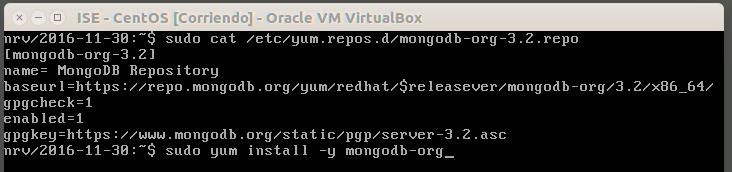
\includegraphics[width=\linewidth]{./Imagenes/P2/O5-1.png}
		\vspace{-0.5cm}
		\caption[Instalación de \textit{MongoDB}.]{Instalación de \textit{MongoDB}.}
		\label{P2-O5-1}
	\end{figure}

	\begin{figure}[H]
		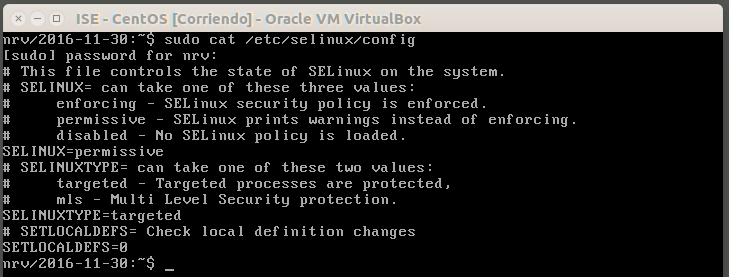
\includegraphics[width=\linewidth]{./Imagenes/P2/O5-2.png}
		\vspace{-0.5cm}
		\caption[Cambio de \textit{SELINUX}.]{Cambio de \textit{SELINUX}.}
		\label{P2-O5-2}
	\end{figure}

	Para entrar en MongoDB ejecutamos \textit{mongo}. Una vez dentro de MongoDB seguimos los siguientes pasos:
	\begin{enumerate}
		\item Creamos la colección que vamos a usar, \textit{Opcional5\_ISE}, para ello ejecutamos \\ \textit{db.createCollection(`Opcional5\_ISE')}.
		\item Creamos dos documentos para luego insertarlos en la colección que hemos creado en el paso anterior. Para ello ejecutamos:
		\begin{enumerate}
			\item \textit{doc = \{ name: ``Nestor'', age: 20 \}}
			\item \textit{doc2 = \{ name: ``NestorJunior'', age: 10 \}}
		\end{enumerate}
		\item Insertamos los documentos en la colección \textit{Opcional5\_ISE}. Para ello ejecutamos:
		\begin{enumerate}
			\item \textit{db.Opcional5\_ISE.insert(doc)}
			\item \textit{db.Opcional5\_ISE.insert(doc2)}
		\end{enumerate}
		\item Finalmente realizamos la consulta en la colección ejecutando \textit{db.Opcional5\_ISE.find()}
	\end{enumerate}

	El resultado de este proceso lo podemos ver en la figura \ref{P2-O5-3}.

	\begin{figure}[H]
		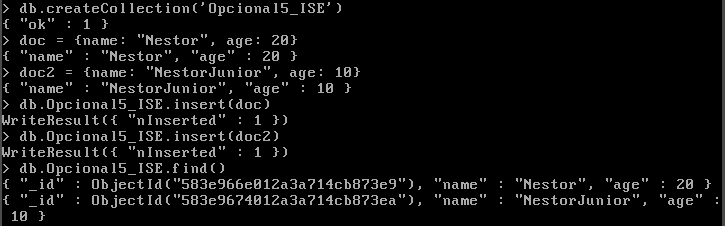
\includegraphics[width=\linewidth]{./Imagenes/P2/O5-3.png}
		\vspace{-0.5cm}
		\caption[Creación de la colección, inserción de documentos y consulta.]{Creación de la colección, inserción de documentos y consulta.}
		\label{P2-O5-3}
	\end{figure}

	\chapter[Práctica 3.]{Práctica 3.}
	
	%%%%%%%%%%%%%%%%%%%%%%%%%%%%%%%%%%%%%%%%%%%%%%%%%%%%
	%%%%%%%%%%%%%%%%%%%% Cuestión Opcional 1 %%%%%%%%%%%
	%%%%%%%%%%%%%%%%%%%%%%%%%%%%%%%%%%%%%%%%%%%%%%%%%%%%
	\section[Cuestión opcional 1: Indique qué comandos ha utilizado para realizarlo así	como capturas de pantalla del proceso de reconstrucción del RAID.]{Cuestión opcional 1: Indique qué comandos ha utilizado para realizarlo así	como capturas de pantalla del proceso de reconstrucción del RAID.}

	Lo que he hecho ha sido seguir la misma idea que en la cuestión opcional 1 de la práctica 1 de esta asignatura. Al igual que en la práctica 1, me he basado en la información que podemos obtener de la Wiki de Linux \cite{raid}. Los pasos que he seguido son los siguientes:

	\begin{enumerate}
	   \item Primero comprobamos que efectivamente tenemos dos RAID. Para ello ejecutamos el comando \textit{cat /proc/mdsatat} como se puede ver en la figura \ref{P3-O1-1}. También se podría haber hecho con \textit{watch -n2 cat /proc/mdstat} pero como no se producen cambios en el fichero, no le sacamos partido a la utilidad \textit{watch}.
	   \item A continuación, producimos un fallo por software en el RAID ejecutando el comando \textit{sudo mdadm -{-}manage -{-}set-faulty /dev/md0 /deb/sdb1} como podemos ver en la figura \ref{P3-O1-2}.
	   \item Retiramos el RAID en caliente ejecutando \textit{sudo mdadm /dev/md0 -r /dev/sdb1} y lo añadimos ejecutando \textit{sudo mdadm /dev/md0 -a /dev/sdb1}, como podemos ver en la figura \ref{P3-O1-3}.
	   \item Ahora si podemos sacarle partido a \textit{watch}. Para comprobar el proceso de recuperación del RAID ejecutamos \textit{watch -n2 cat /proc/mdstat}. De este modo, cada dos segundos se ejecutará \textit{cat /proc/mdstat}, proporcionándonos así una idea de como va el progreso, como se puede ver en la figura \ref{P3-O1-4}.
	   \item Tras un tiempo de recuperación, el RAID se ha recuperado correctamente y vuelve a estar en funcionamiento, como podemos ver en la figura \ref{P3-O1-5}.
	\end{enumerate}

	\begin{figure}[H]
	   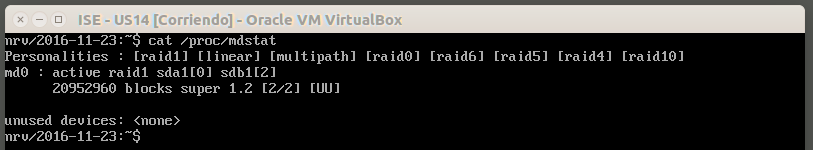
\includegraphics[width=\linewidth]{./Imagenes/P3/O1-1.png}
	   \vspace{-0.5cm}
	   \caption[Comprobamos que tenemos dos RAID.]{Comprobamos que tenemos dos RAID.}
	   \label{P3-O1-1}
	\end{figure}

	\begin{figure}[H]
	   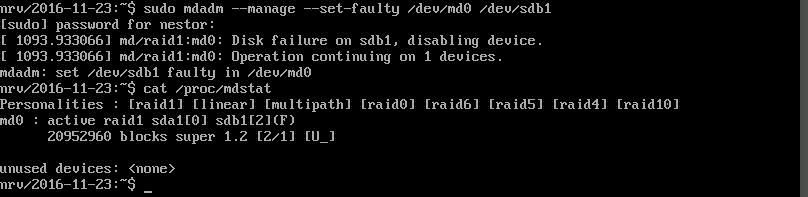
\includegraphics[width=\linewidth]{./Imagenes/P3/O1-2.png}
	   \vspace{-0.5cm}
	   \caption[Provocamos un fallo software en el RAID.]{Provocamos un fallo software en el RAID.}
	   \label{P3-O1-2}
	\end{figure}

	\begin{figure}[H]
	   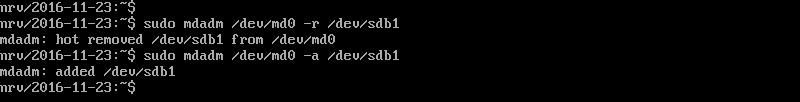
\includegraphics[width=\linewidth]{./Imagenes/P3/O1-3.png}
	   \vspace{-0.5cm}
	   \caption[Quitamos en caliente y añadimos de nuevo el RAID.]{Quitamos en caliente y añadimos de nuevo el RAID.}
	   \label{P3-O1-3}
	\end{figure}

	\begin{figure}[H]
	   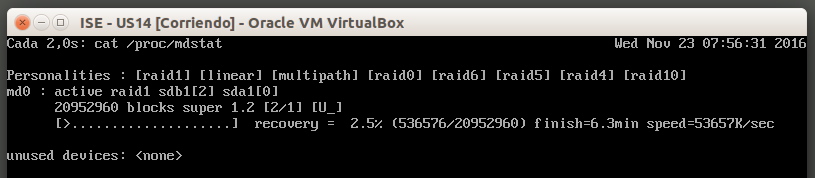
\includegraphics[width=\linewidth]{./Imagenes/P3/O1-4.png}
	   \vspace{-0.5cm}
	   \caption[Observamos el proceso de recuperación con \textit{watch}.]{Observamos el proceso de recuperación con \textit{watch}.}
	   \label{P3-O1-4}
	\end{figure}

	\begin{figure}[H]
	   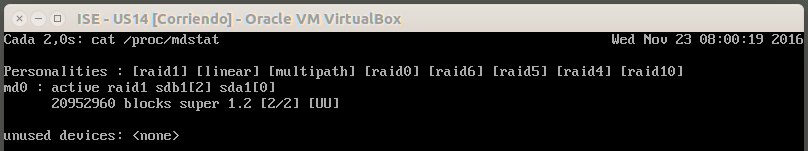
\includegraphics[width=\linewidth]{./Imagenes/P3/O1-5.png}
	   \vspace{-0.5cm}
	   \caption[RAID completamente restaurado.]{RAID completamente restaurado.}
	   \label{P3-O1-5}
	\end{figure}

	%%%%%%%%%%%%%%%%%%%%%%%%%%%%%%%%%%%%%%%%%%%%%%%%%%%%
	%%%%%%%%%%%%%%%%%%%% Cuestión Opcional 2 %%%%%%%%%%%
	%%%%%%%%%%%%%%%%%%%%%%%%%%%%%%%%%%%%%%%%%%%%%%%%%%%%
	\section[Cuestión opcional 2: Instale Nagios en su sistema (el que prefiera) documentando el proceso y muestre el resultado de la monitorización de su sistema comentando qué aparece.]{Cuestión opcional 2: Instale Nagios en su sistema (el que prefiera) documentando el proceso y muestre el resultado de la monitorización de su sistema comentando qué aparece.}

	El proceso de instalación lo podemos ver en la página oficial de Nagios \cite{nagios}. Yo lo voy a hacer en CentOS. Los pasos a seguir son:

	\begin{enumerate}
	   \item El proceso de instalacion se hace desde el directorio \textit{/tmp}, así que ejecutamos \textit{cd /tmp} para irnos a dicha carpeta, como podemos ver en la figura \ref{P3-O2-1}.
	   \item Descargamos la última versión de \textit{Nagios}. Para ello ejecutamos el comando \textit{wget http://assets.nagios.com/downloads/nagiosxi/xi-latest.tar.gz}, como podemos ver en la figura \ref{P3-O2-1}.
	   \item Descomprimimos Nagios ejecutando \textit{tar xzf xi-latest.tar.gz}, como podemos ver en la figura \ref{P3-O2-1}.
	   \item Nos vamos a la carpeta que se ha creado ejecutando \textit{cd /tmp/nagiosxi}, como podemos ver en la figura \ref{P3-O2-2}.
	   \item Ejecutamos el script de instalación con el comando \textit{sudo ./fullinstalation}\footnote{Cuidado: este script cambia la contraseña del usuario root de MySQL a \textit{nagiosxi}}, como podemos ver en la figura \ref{P3-O2-2}. Nos preguntara si queremos continuar, le decimos que sí pulsando la tecla \textit{y}.
	\end{enumerate}

	\begin{figure}[H]
	   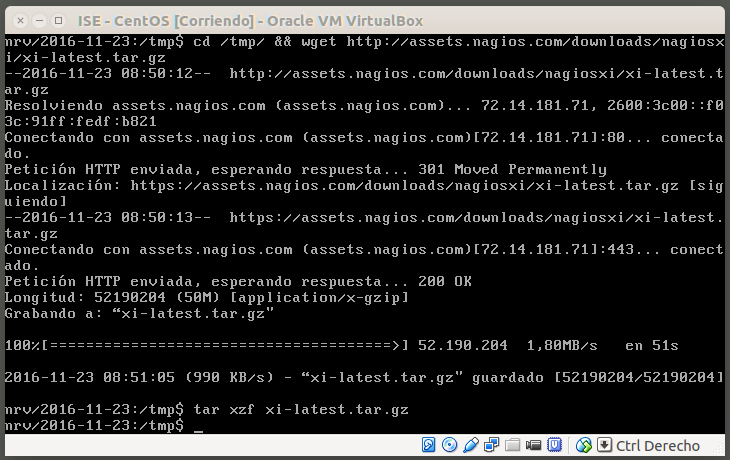
\includegraphics[width=\linewidth]{./Imagenes/P3/O2-1.png}
	   \vspace{-0.5cm}
	   \caption[Proceso de descarga de Nagios y preparación para la instalación.]{Proceso de descarga de Nagios y preparación para la instalación.}
	   \label{P3-O2-1}
	\end{figure}

	\begin{figure}[H]
	   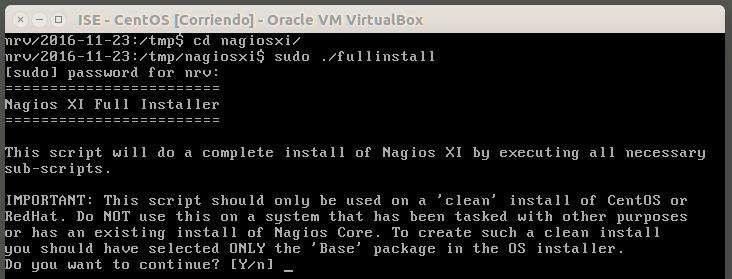
\includegraphics[width=\linewidth]{./Imagenes/P3/O2-2.png}
	   \vspace{-0.5cm}
	   \caption[Proceso de instalación de Nagios.]{Proceso de instalación de Nagios.}
	   \label{P3-O2-2}
	\end{figure}

	Una vez hemos instalado Nagios, en el manual de instalación \cite{nagios} podemos ver que para acceder a Nagios desde mi máquina anfitriona debemos poner en el buscador \textit{http://IP/nagios}, donde \textit{IP} es la dirección del servidor al que nos queremos conectar. En mi caso, la dirección IP es \textit{192.168.56.101}, como podemos ver en la figura \ref{P3-O2-conexion}. Tras introducir la dirección en el navegador, podemos ver que nos conectamos correctamente a Nagios, como se puede ver en la figura \ref{P3-O2-conexion}.

	\begin{figure}[H]
	   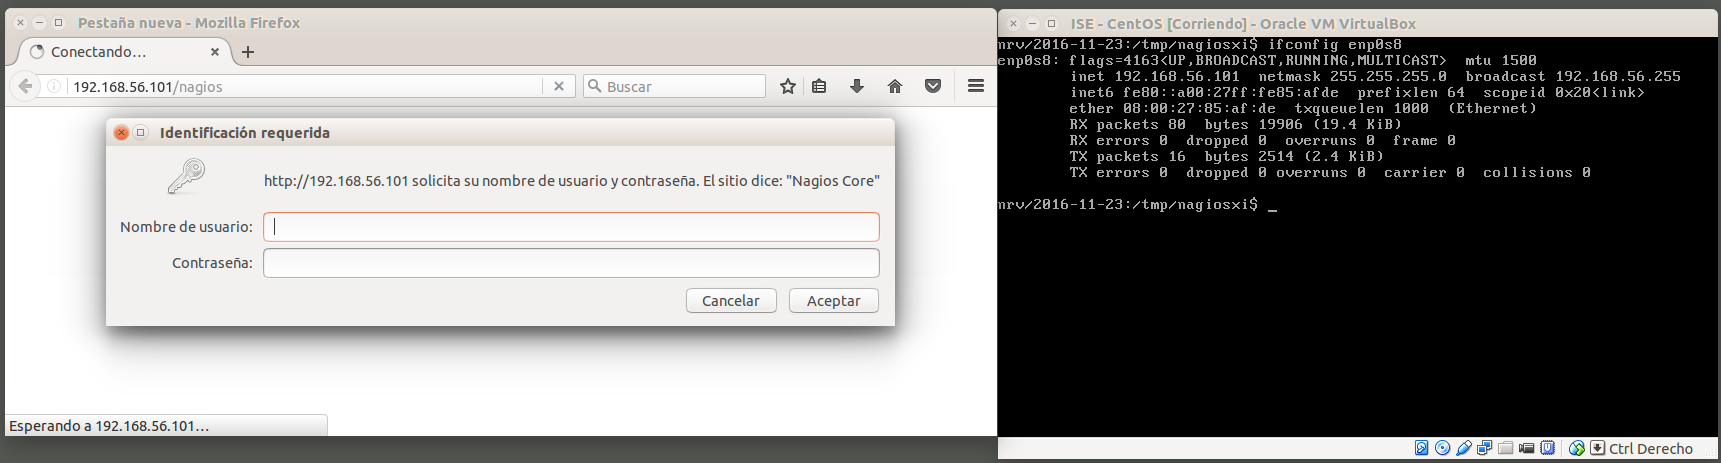
\includegraphics[width=\linewidth]{./Imagenes/P3/O2-conexion.png}
	   \vspace{-0.5cm}
	   \caption[Conexión con Nagios (máquina conectadas en modo \textit{host-only}).]{Conexión con Nagios (máquina conectadas en modo \textit{host-only}).}
	   \label{P3-O2-conexion}
	\end{figure}

	Vemos que nos pide una contraseña. Para poder acceder debemos seguir los pasos que nos indica Nagios en su guía para configurar la interfaz web \cite{nagios2}. Debemos acceder a la dirección de nuestro servidor, como podemos ver en la figura \ref{P3-O2-web1}. Una vez en dicha página, le damos a acceder y ahí configuramos nuestros datos, como podemos ver en la figura \ref{P3-O2-web2}. A continuación, pulsamos \textit{install}.

	\begin{figure}[H]
	   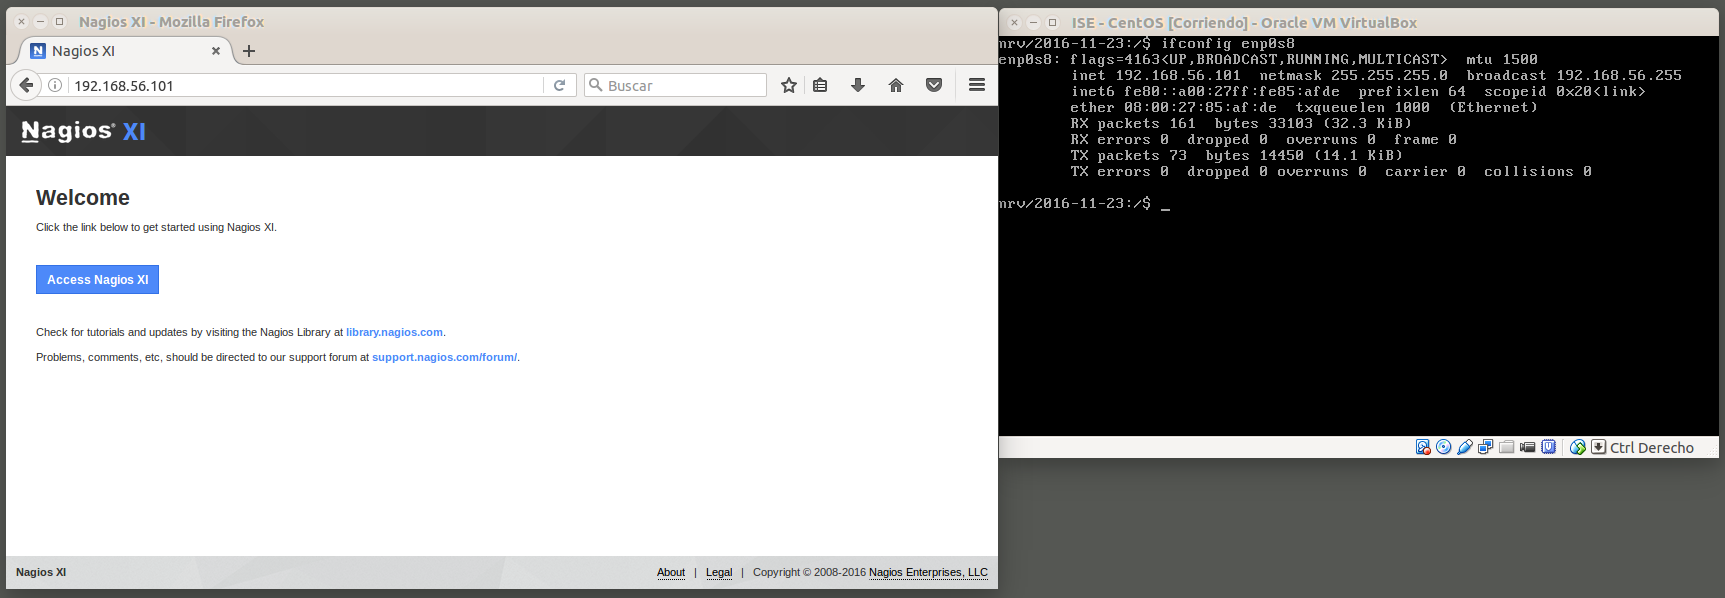
\includegraphics[width=\linewidth]{./Imagenes/P3/O2-web1.png}
	   \vspace{-0.5cm}
	   \caption[Paso 1 de la configuración de la interfaz web (máquina conectadas en modo \textit{host-only}).]{Paso 1 de la configuración de la interfaz web (máquina conectadas en modo \textit{host-only}).}
	   \label{P3-O2-web1}
	\end{figure}

	\begin{figure}[H]
	   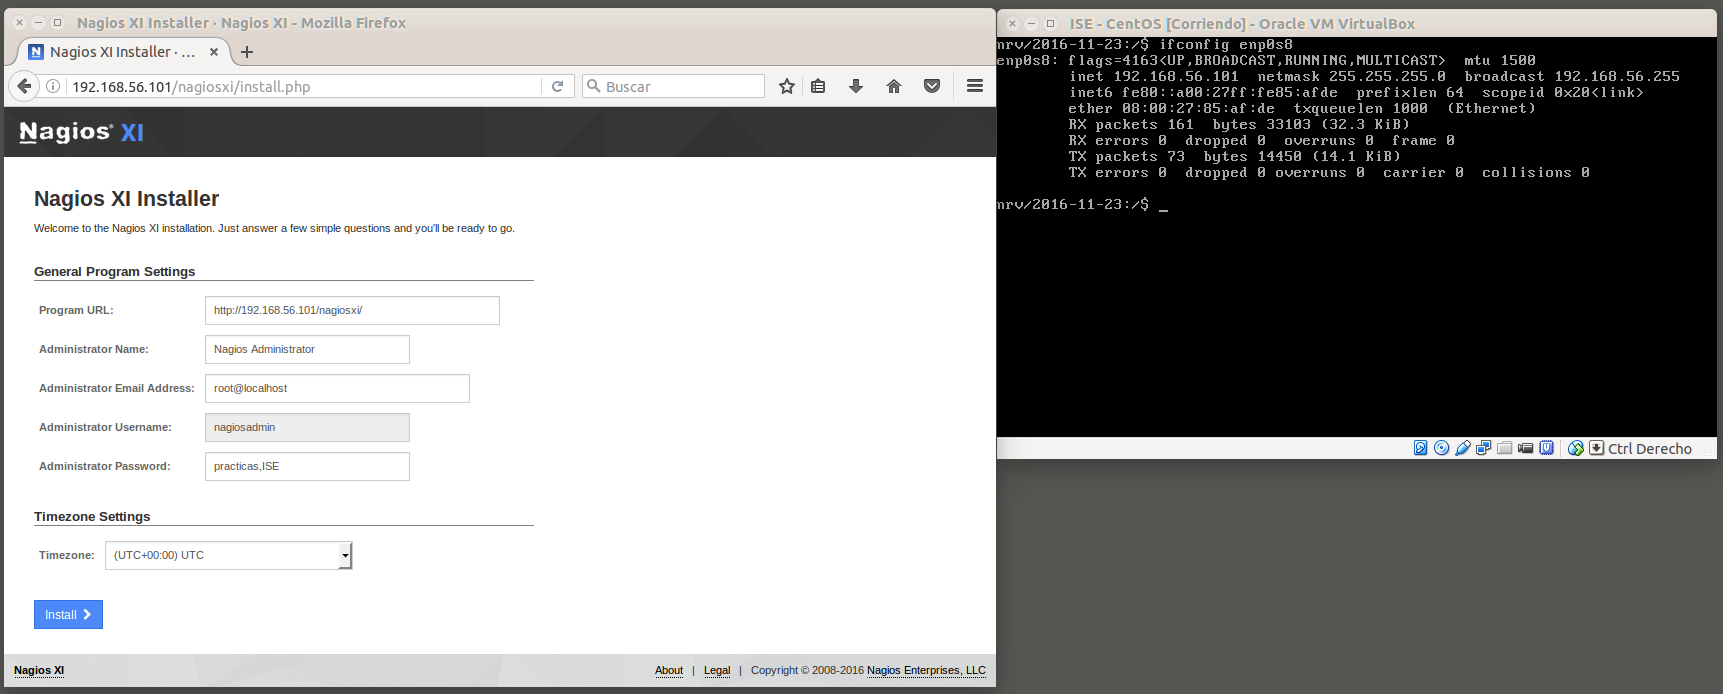
\includegraphics[width=\linewidth]{./Imagenes/P3/O2-web2.png}
	   \vspace{-0.5cm}
	   \caption[Paso 2 de la configuración de la interfaz web (máquina conectadas en modo \textit{host-only}).]{Paso 2 de la configuración de la interfaz web (máquina conectadas en modo \textit{host-only}).}
	   \label{P3-O2-web2}
	\end{figure}

	Ahora si podemos acceder usando los datos que hemos introducido en el paso anterior (ver figura \ref{P3-O2-web2}), como podemos ver en la figura \ref{P3-O2-conexion2}.

	\begin{figure}[H]
	   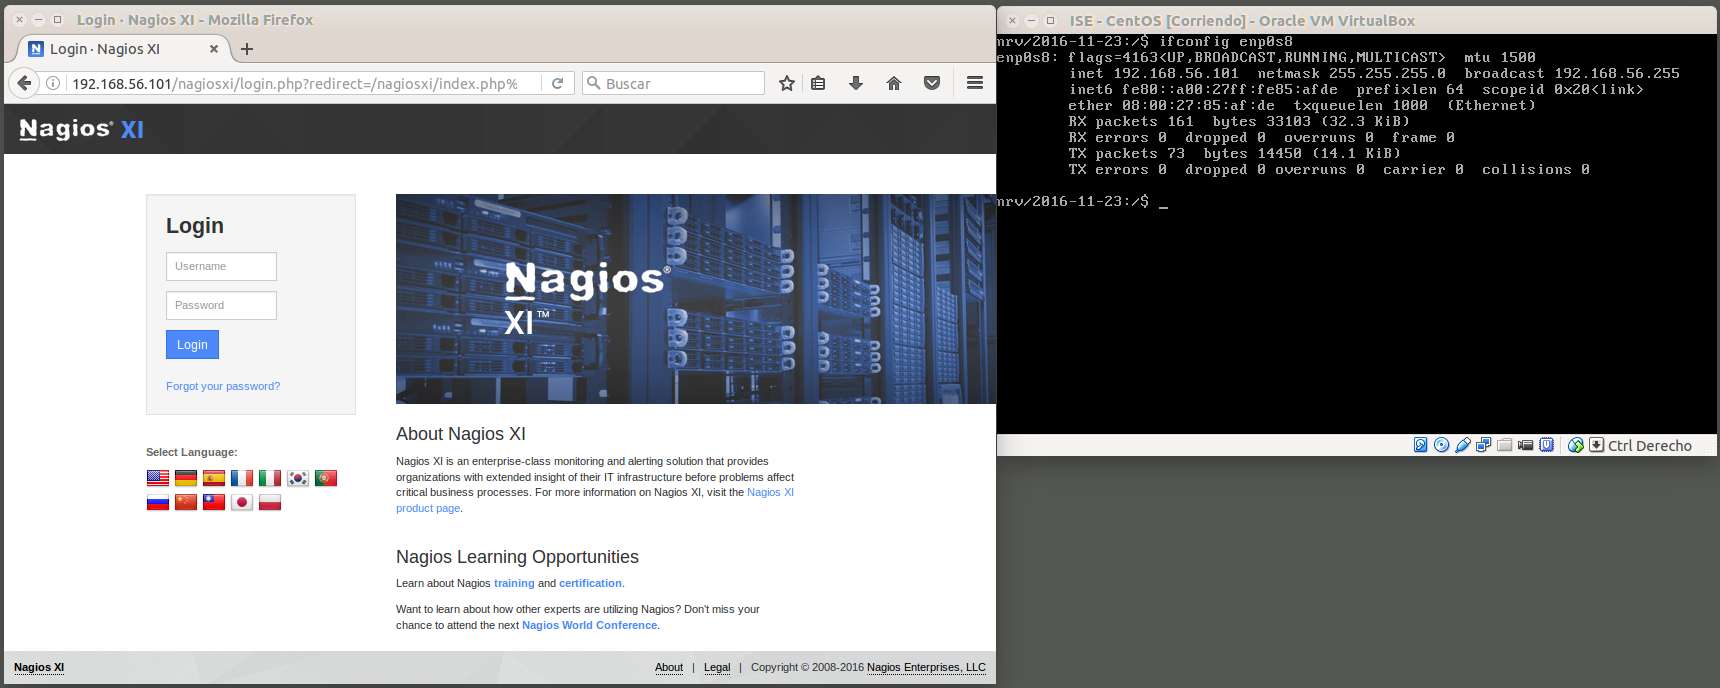
\includegraphics[width=\linewidth]{./Imagenes/P3/O2-conexion2.png}
	   \vspace{-0.5cm}
	   \caption[Conexión con Nagios (máquina conectadas en modo \textit{host-only}).]{Conexión con Nagios (máquina conectadas en modo \textit{host-only}).}
	   \label{P3-O2-conexion2}
	\end{figure}

	Una vez hemos accedido a Nagios podemos ver que se pueden monitorizar diferentes parámetros. Como la mayoría de monitores, nos permite monitorizar el rendimiento de nuestro servidor, como podemos ver en la figura \ref{P3-O2-rendimiento}. Una de las características que más me ha llamado la atención es la llamada \textit{Hypermap}. Esta opción nos muestra un mapa con el estado actual de los dispositivos de red (hosts), como podemos ver en la figura \ref{P3-O2-hypermap}.

	\begin{figure}[H]
	   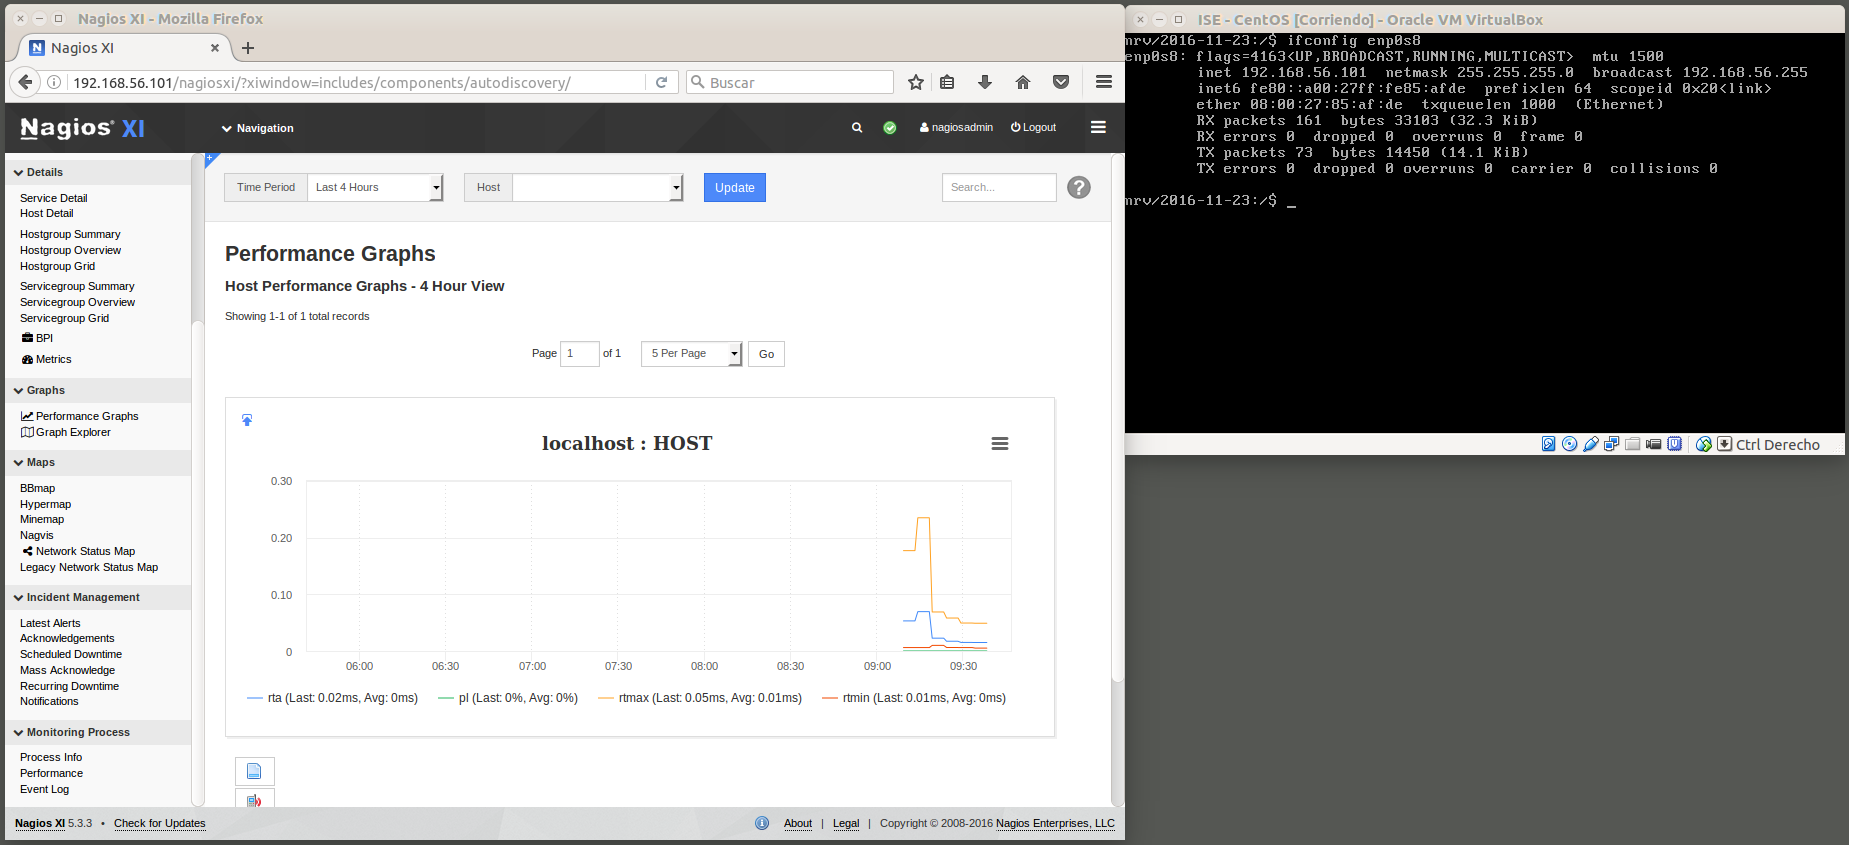
\includegraphics[width=\linewidth]{./Imagenes/P3/O2-rendimiento.png}
	   \vspace{-0.5cm}
	   \caption[Monitorización del rendimiento con Nagios (máquina conectadas en modo \textit{host-only}).]{Monitorización del rendimiento con Nagios (máquina conectadas en modo \textit{host-only}).}
	   \label{P3-O2-rendimiento}
	\end{figure}

	\begin{figure}[H]
	   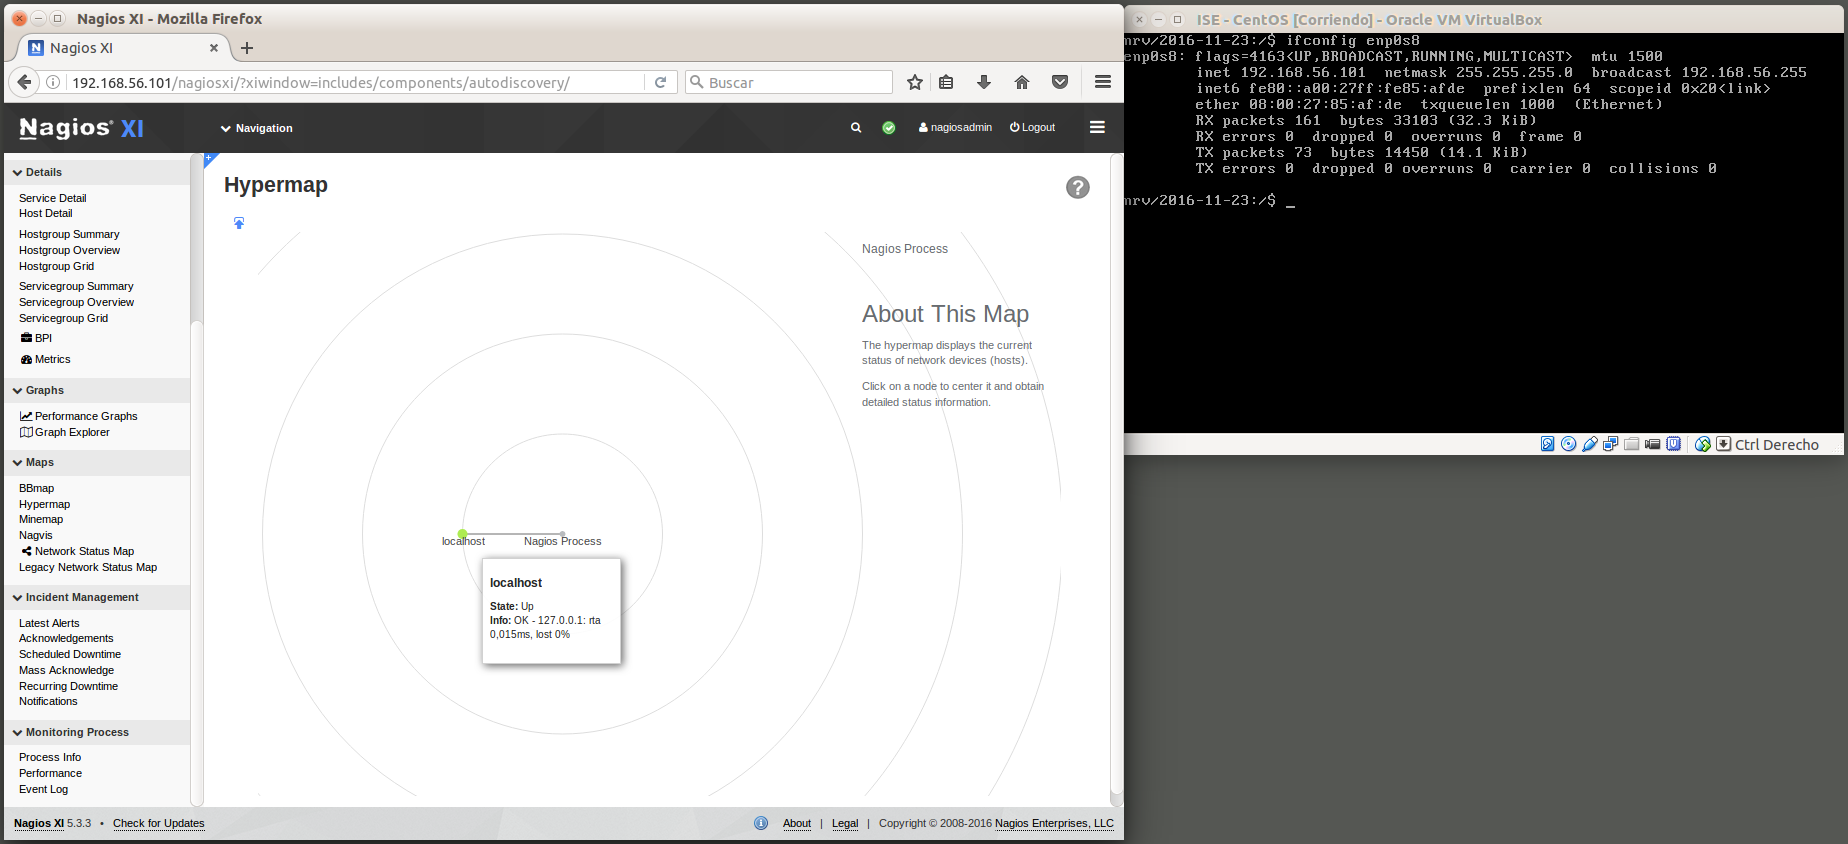
\includegraphics[width=\linewidth]{./Imagenes/P3/O2-hypermap.png}
	   \vspace{-0.5cm}
	   \caption[Hypermap de mi servidor (máquina conectadas en modo \textit{host-only}).]{Hypermap de mi servidor  (máquina conectadas en modo \textit{host-only}).}
	   \label{P3-O2-hypermap}
	\end{figure}

	%%%%%%%%%%%%%%%%%%%%%%%%%%%%%%%%%%%%%%%%%%%%%%%%%%%%
	%%%%%%%%%%%%%%%%%%%% Cuestión Opcional 4 %%%%%%%%%%%
	%%%%%%%%%%%%%%%%%%%%%%%%%%%%%%%%%%%%%%%%%%%%%%%%%%%%
	\section[Cuestión opcional 4: Pruebe a instalar este monitor en alguno de sus tres sistemas. Realice capturas de pantalla del proceso de instalación y comente capturas de pantalla del programa en ejecución.]{Cuestión opcional 4: Pruebe a instalar este monitor en alguno de sus tres sistemas. Realice capturas de pantalla del proceso de instalación y comente capturas de pantalla del programa en ejecución.}

	Voy a instalar \textit{Zabbix} en Ubuntu Server siguiendo los pasos que nos indica Digital Ocean \cite{zabbix}. Los pasos a seguir para la instalación son: \label{P3-pasos_zabbix}
	\begin{enumerate}
	   \item \textit{Zabbix} se encuentra en los repositorios de Ubuntu, pero está desactualizado, por ello vamos a instalarlo desde los repositorios del programa. Para ello, editamos el fichero \textit{/etc/apt/sources.list} y añadimos las líneas: \\

	   \# Zabbix Application PPA \\
	   deb http://ppa.launchpad.net/tbfr/zabbix/ubuntu precise main \\
	   deb-src http://ppa.launchpad.net/tbfr/zabbix/ubuntu precise main \\

	   El archivo quedaría como podemos ver en la figura \ref{P3-O4-1}.
	   \item A continuación añadimos la clave del PPA para que \textit{apt} confíe en la fuente. Para ello ejecutamos: \textit{sudo apt-key adv -{-}keyserver keyserver.ubuntu.com -{-}recv-keys C407E17D5F76A32B}, como podemos ver en la figura \ref{P3-O4-2}.
	   \item Una vez hecho esto, actualizamos los repositorios con \textit{sudo apt-get update} e instalamos \textit{Zabbix} ejecutando \textit{sudo apt-get install zabbix-server-mysql php5-mysql zabbix-frontend-php}, como podemos ver en la figura \ref{P3-O4-2}.
	\end{enumerate}

	\begin{figure}[H]
	   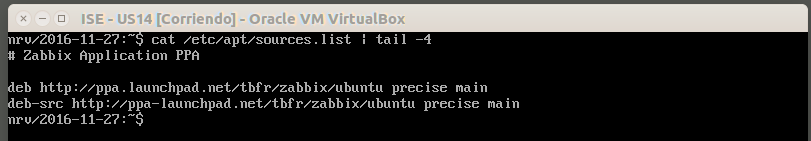
\includegraphics[width=\linewidth]{./Imagenes/P3/O4-1.png}
	   \vspace{-0.5cm}
	   \caption[Archivo \textit{/etc/apt/sources.list}.]{Archivo \textit{/etc/apt/sources.list}.}
	   \label{P3-O4-1}
	\end{figure}

	\begin{figure}[H]
	   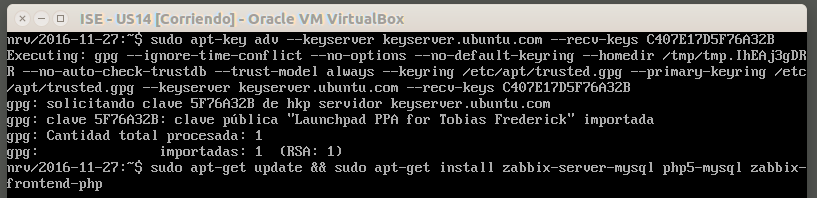
\includegraphics[width=\linewidth]{./Imagenes/P3/O4-2.png}
	   \vspace{-0.5cm}
	   \caption[Instalación de \textit{Zabbix}.]{Instalación de \textit{Zabbix}.}
	   \label{P3-O4-2}
	\end{figure}

	Los siguiente que debemos hacer es configurar el server de \textit{Zabbix}, para ello editamos el archivo \textit{/etc/zabbix/zabbix\_server.conf}, y cambiamos el valor de \textit{DBName}, \textit{DBUser} y\textit{DBPassword}. Dichos parámetros han quedado como podemos ver en la figura \ref{P3-O4-3}.

	\begin{figure}[H]
	   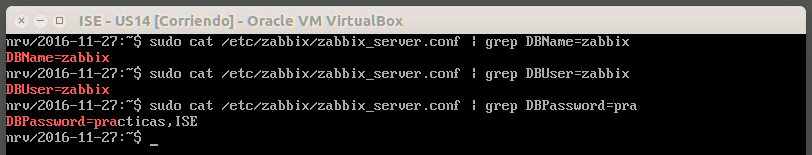
\includegraphics[width=\linewidth]{./Imagenes/P3/O4-3.png}
	   \vspace{-0.5cm}
	   \caption[Configuración del servidor de \textit{Zabbix}.]{Configuración del servidor \textit{Zabbix}.}
	   \label{P3-O4-3}
	\end{figure}

	A continuación configuramos MySQL. Para ello seguimos los siguientes pasos:
	\begin{enumerate}
	   \item Extramos los ficheros SQL del directorio \textit{cd /usr/share/zabbix-server-mysql/} ejecutando \textit{sudo gunzip *.gz}, como podemos ver en la figura \ref{P3-O4-4}.
	   \item Entramos a MySQL como usuarios root ejecutando \textit{mysql -u root -p}, como podemos ver en la figura \ref{P3-O4-5}.
	   \item Creamos un usuario para \textit{Zabbix} que coincida con los datos que escribimos en el fichero \textit{/etc/zabbix/zabbix\_server.conf} ejecutando \textit{create user `zabbix'@`localhost' identified by `practicas,ISE';}, como podemos ver en la figura \ref{P3-O4-5}.
	   \item Creamos una base de datos para \textit{Zabbix} ejecutando \textit{create database zabbix;}, como podemos ver en la figura \ref{P3-O4-5}.
	   \item Le damos permisos sobre dicha base de datos al usuario que hemos creado con anterioridad ejecutando \textit{grant all privileges on zabbix.* to `zabbix'@`localhost';}, como podemos ver en la figura \ref{P3-O4-5}.
	   \item Actualizamos los permisos ejecutando \textit{flush privileges;}, como podemos ver en la figura \ref{P3-O4-5}.
	   \item Salimos de MySQL ejecutando \textit{exit;}, como podemos ver en la figura \ref{P3-O4-5}.
	   \item Importamos los archivos que \textit{Zabbix} necesita para funcionar, para ello y como podemos ver en la figura \ref{P3-O4-6}, ejecutamos:
	      \begin{itemize}
	         \item \textit{mysql -u zabbix -p zabbix $<$ schema.sql}
	         \item \textit{mysql -u zabbix -p zabbix $<$ images.sql}
	         \item \textit{mysql -u zabbix -p zabbix $<$ data.sql}
	      \end{itemize}
	\end{enumerate}

	\begin{figure}[H]
	   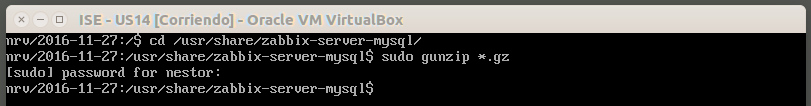
\includegraphics[width=\linewidth]{./Imagenes/P3/O4-4.png}
	   \vspace{-0.5cm}
	   \caption[Extracción de ficheros SQL.]{Extracción de ficheros SQL.}
	   \label{P3-O4-4}
	\end{figure}

	\begin{figure}[H]
	   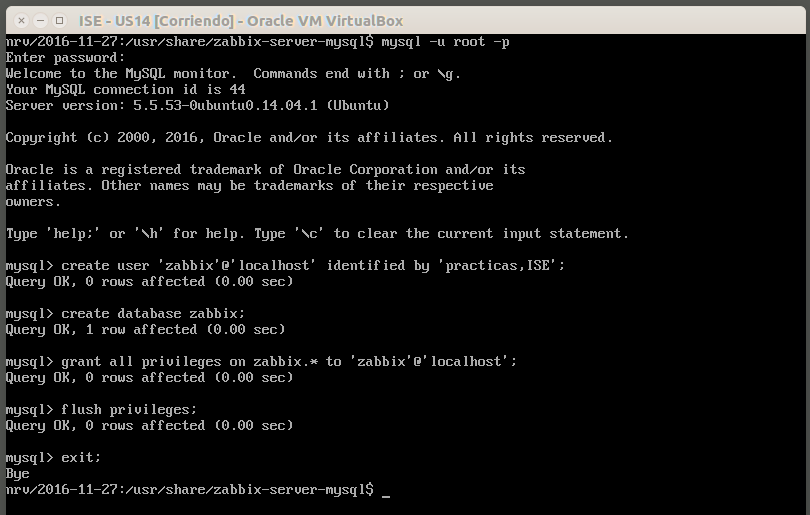
\includegraphics[width=\linewidth]{./Imagenes/P3/O4-5.png}
	   \vspace{-0.5cm}
	   \caption[Configuración de MySQL.]{Configuración de MySQL.}
	   \label{P3-O4-5}
	\end{figure}

	\begin{figure}[H]
	   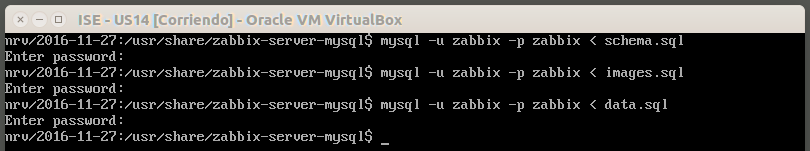
\includegraphics[width=\linewidth]{./Imagenes/P3/O4-6.png}
	   \vspace{-0.5cm}
	   \caption[Importación de archivos necesarios para \textit{Zabbix}.]{Importación de archivos necesarios para \textit{Zabbix}.}
	   \label{P3-O4-6}
	\end{figure}

	Una vez hemos configurado MySQL, pasamos a la configuración de PHP. Para ello editamos el fichero \textit{/etc/php5/apache2/php.ini}. Buscamos y modificamos los siguientes parámetros para que queden como a continuación:

	\begin{itemize}
	   \item post\_max\_size = 16M
	   \item max\_execution\_time = 300
	   \item max\_input\_time = 300
	   \item date.timezone = UTC
	\end{itemize}

	El resultado lo podemos ver en la figura \ref{P3-O4-7}.

	\begin{figure}[H]
	   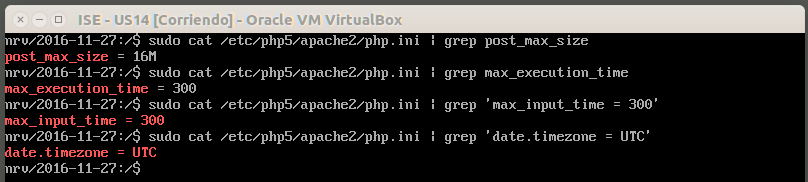
\includegraphics[width=\linewidth]{./Imagenes/P3/O4-7.png}
	   \vspace{-0.5cm}
	   \caption[Parámetros del archivo \textit{/etc/php5/apache2/php.ini} modificados.]{Parámetros del archivo \textit{/etc/php5/apache2/php.ini} modificados.}
	   \label{P3-O4-7}
	\end{figure}

	Copiamos el archivo de configuración de php específico de \textit{Zabbix} ejecutando \textit{sudo cp /usr/share/doc/zabbix-frontend-php/examples/zabbix.conf.php.example /etc/zabbix/zabbix.conf.php} para poder ejecutarlo y cambiar los parámetros que podemos ver a continuación para que queden de la siguiente manera:
	\begin{itemize}
	   \item \$DB[``DATABASE''] = `zabbix';
	   \item \$DB[``USER''] = `zabbix';
	   \item \$DB[``PASSWORD''] = `practicas,ISE'
	\end{itemize}

	El resultado lo podemos ver en la figura \ref{P3-O4-8}.

	\begin{figure}[H]
	   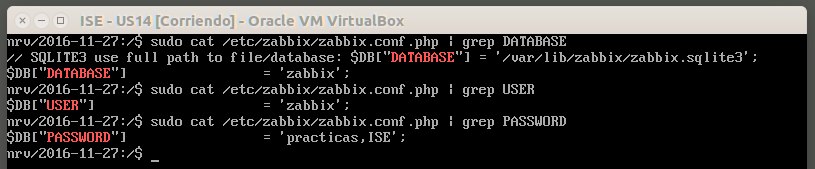
\includegraphics[width=\linewidth]{./Imagenes/P3/O4-8.png}
	   \vspace{-0.5cm}
	   \caption[Parámetros del archivo \textit{/etc/zabbix/zabbix.conf.php} modificados.]{Parámetros del archivo \textit{/etc/zabbix/zabbix.conf.php} modificados.}
	   \label{P3-O4-8}
	\end{figure}

	A continuación copiamos el archivo apache de \textit{Zabbix} en los archivos de configuración de apache ejecutando. Para ello ejecutamos:
	\begin{itemize}
	   \item \textit{sudo cp /usr/share/doc/zabbix-frontend-php/examples/apache.conf /etc/apache2/\\conf-aviable/zabbix.conf}
	   \item \textit{sudo cp /usr/share/doc/zabbix-frontend-php/examples/apache.conf /etc/apache2/\\conf-enable/zabbix.conf}
	\end{itemize}

	Nos aseguramos de que los alias están habilitados dentro de Apache ejecutando \textit{sudo a2enmod alias} y reiniciamos \textit{Apache} ejecutando \textit{sudo service apache2 restart}. Todo este proceso lo podemos ver en la figura \ref{P3-O4-9}. Lo siguiente que tenemos que hacer es editar el fichero \textit{/etc/default/zabbix-server} y cambiar el valor de \textit{START} a ``yes'' e iniciamos \textit{Zabbix} ejecutando \textit{sudo service zabbix-server start} como podemos ver en la figura \ref{P3-O4-10}.

	\begin{figure}[H]
	   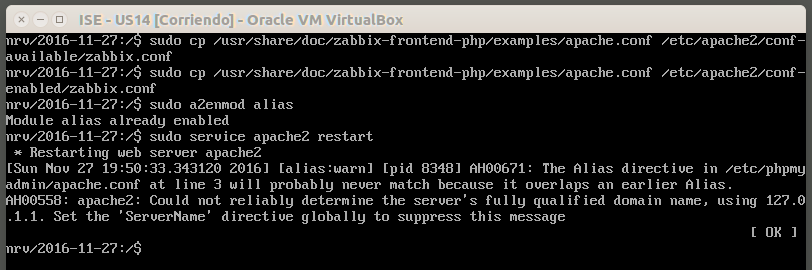
\includegraphics[width=\linewidth]{./Imagenes/P3/O4-9.png}
	   \vspace{-0.5cm}
	   \caption[Configuración archivo apache de \textit{Zabbix}.]{Configuración archivo apache de \textit{Zabbix}.}
	   \label{P3-O4-9}
	\end{figure}

	\begin{figure}[H]
	   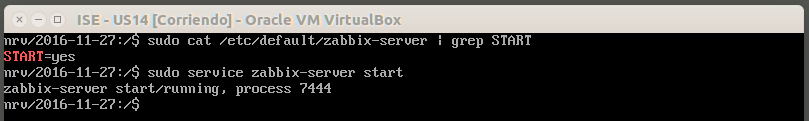
\includegraphics[width=\linewidth]{./Imagenes/P3/O4-10.png}
	   \vspace{-0.5cm}
	   \caption[Inicio de \textit{Zabbix}.]{Inicio de \textit{Zabbix}.}
	   \label{P3-O4-10}
	\end{figure}

	Ya está todo listo en el servidor, ahora debemos configurar el cliente. El cliente en mi caso va a ser mi máquina anfitriona. Debemos instalar el \textit{Agente de Zabbix}, para ello seguimos los 2 primeros pasos que realizamos en el servidor \ref{P3-pasos_zabbix}, como podemos ver en la figura \ref{P3-O4-11}. A continuación instalamos el \textit{Agente de Zabbix} ejecutando \textit{sudo apt-get install zabbix-agent}.

	\begin{figure}[H]
	   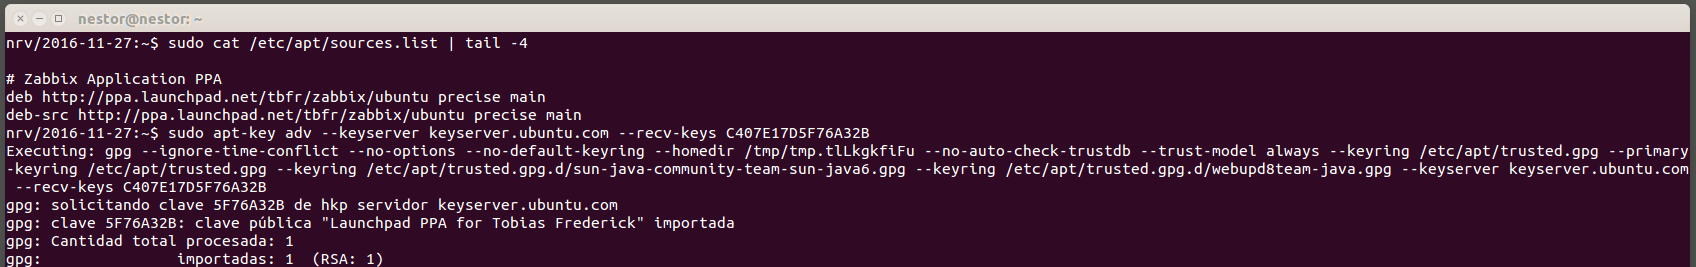
\includegraphics[width=\linewidth]{./Imagenes/P3/O4-11.png}
	   \vspace{-0.5cm}
	   \caption[Instalación del \textit{Agente de Zabbix}.]{Instalación del \textit{Agente de Zabbix}.}
	   \label{P3-O4-11}
	\end{figure}

	Una vez instalado, pasamos a modificar los archivos de configuración. El primero de ellos es \textit{/etc/zabbix/zabbix\_agentd.conf}. Como podemos ver en la figura \ref{P3-O4-12} la dirección IP de mi servidor es \textit{192.168.56.103} así que en dicho archivo, en el parámetro \textit{Server} debemos poner dicha dirección, como se ve en la figura \ref{P3-O4-12} y reiniciamos el servicio ejecutando \textit{sudo service zabbix-agent restart}.

	\begin{figure}[H]
	   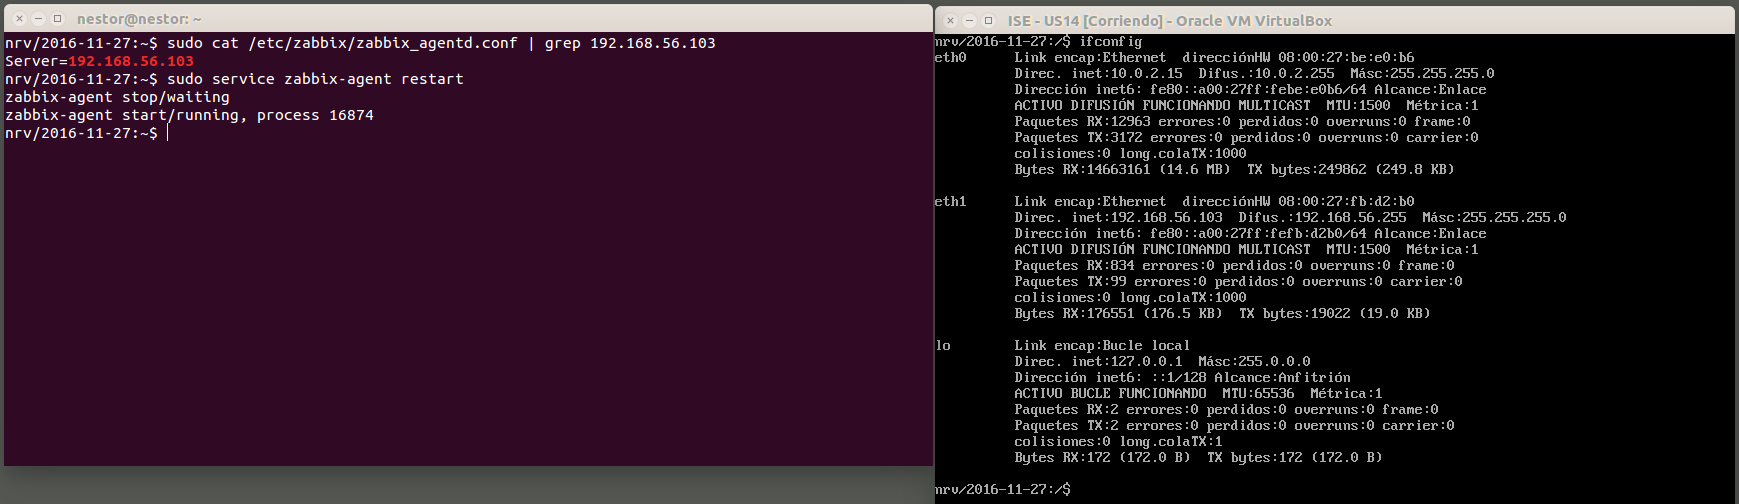
\includegraphics[width=\linewidth]{./Imagenes/P3/O4-12.png}
	   \vspace{-0.5cm}
	   \caption[Dirección IP del servidor con \textit{Zabbix} instalado (máquinas conectadas en modo \textit{host-only}).]{Dirección IP del servidor con \textit{Zabbix} instalado (máquinas conectadas en modo \textit{host-only}).}
	   \label{P3-O4-12}
	\end{figure}

	Dentro del mismo fichero debemos editar el valor de \textit{Hostname} y poner el \textit{hostname} de la máquina cliente, \textit{nestor} en mi caso, y reiniciamos el servicio, como podemos ver en la figura \ref{P3-O4-13}

	\begin{figure}[H]
	   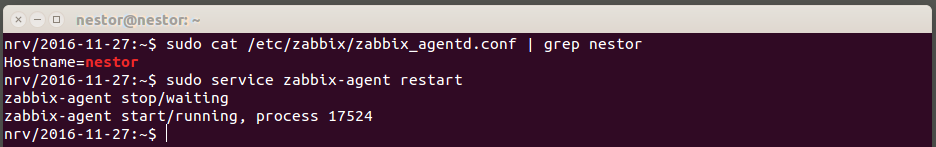
\includegraphics[width=\linewidth]{./Imagenes/P3/O4-13.png}
	   \vspace{-0.5cm}
	   \caption[Parámetro \textit{hostname}.]{Parámetro \textit{hostname}.}
	   \label{P3-O4-13}
	\end{figure}

	Finalmente, para acceder al servicio debemos escribir en la barra del navegador la dirección IP de nuestro servidor seguido de \textit{/zabbix}, como podemos ver en la figura \ref{P3-O4-14}. Por defecto, el usuario y contraseña para entrar son \textit{admin} y \textit{zabbix} respectivamente.

	\begin{figure}[H]
	   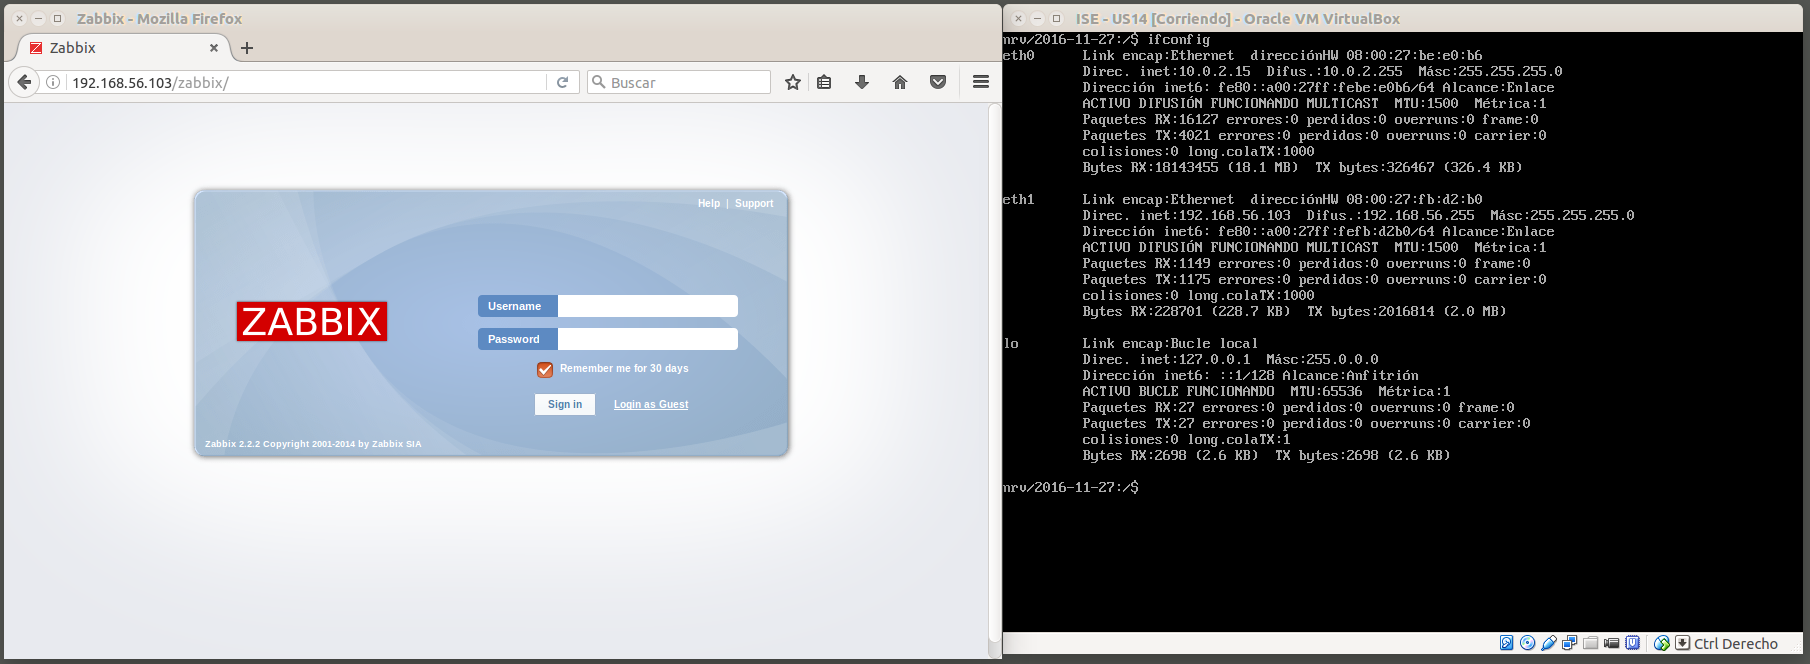
\includegraphics[width=\linewidth]{./Imagenes/P3/O4-14.png}
	   \vspace{-0.5cm}
	   \caption[\textit{Zabbix} en funcionamiento.]{\textit{Zabbix} en funcionamiento}
	   \label{P3-O4-14}
	\end{figure}

	Una vez hemos entrado, nos vamos a la pestaña \textit{Configuration} y dentro de dicha pestaña elegimos la de \textit{Hosts}, como podemos ver la figura \ref{P3-O4-15}. Una vez aquí, pinchamos sobre \textit{Zabbix Server}.

	\begin{figure}[H]
	   \includegraphics[width=\linewidth]{./Imagenes/P3/O4-15.png}
	   \vspace{-0.5cm}
	   \caption[Host disponibles.]{Host disponibles.}
	   \label{P3-O4-15}
	\end{figure}

	Dentro del servidor de \textit{Zabbix}, al final de todo, en la sección de \textit{Status} elegimos \textit{Monitored}, como podemos ver en la figura \ref{P3-O4-16}.

	\begin{figure}[H]
	   \includegraphics[width=\linewidth]{./Imagenes/P3/O4-16.png}
	   \vspace{-0.5cm}
	   \caption[Cambio del estado del servidor.]{Cambio del estado del servidor.}
	   \label{P3-O4-16}
	\end{figure}

	Tras unos instantes, podemos ver que en la pestaña \textit{Last data} dentro de \textit{Monitorig} los distintos hosts que se pueden modificar. Dentro de nuestro servidor \textit{Zabbix}, podemos ver una gran cantidad de parámetros monitorizados. Parte de ellos los podemos ver en la figura \ref{P3-O4-17}.

	\begin{figure}[H]
	   \includegraphics[width=\linewidth]{./Imagenes/P3/O4-17.png}
	   \vspace{-0.5cm}
	   \caption[Parámetros monitorizados.]{Parámetros monitorizados.}
	   \label{P3-O4-17}
	\end{figure}

	Uno de los parámetros que podemos ver es el número de valores procesados por el servidor \textit{Zabbix} por segundo. Podemos ver una gráfica sobre la información recogida de dicho parámetro en la figura \ref{P3-O4-18}. En dicha gráfica podemos ver que no hay mucha actividad en el servidor. El servidor se ha puesto en marcha a las 23:14 y la gráfica llega hasta las 23:36. En este periodo el valor se mantiene ``constante'' en un valor algo superior a 0.38. Podemos ver que hay dos picos a las 23:18 y 23:28 con un valor cercano a 0.42 valores procesados por el servidor \textit{Zabbix} por segundo.

	\begin{figure}[H]
	   \includegraphics[width=\linewidth]{./Imagenes/P3/O4-18.png}
	   \vspace{-0.5cm}
	   \caption[Valores procesados por el servidor \textit{Zabbix} por segundo.]{Valores procesados por el servidor \textit{Zabbix} por segundo.}
	   \label{P3-O4-18}
	\end{figure}

	%%%%%%%%%%%%%%%%%%%%%%%%%%%%%%%%%%%%%%%%%%%%%%%%%%%%
	%%%%%%%%%%%%%%%%%%%% Cuestión Opcional 5 %%%%%%%%%%%
	%%%%%%%%%%%%%%%%%%%%%%%%%%%%%%%%%%%%%%%%%%%%%%%%%%%%
	\section[Cuestión opcional 5: Pruebe a instalar este monitor en alguno de sus tres sistemas. Realice capturas de pantalla del proceso de instalación y comente capturas de pantalla del programa en ejecución.]{Cuestión opcional 5: Pruebe a instalar este monitor en alguno de sus tres sistemas. Realice capturas de pantalla del proceso de instalación y comente capturas de pantalla del programa en ejecución.}

	La instalación voy a hacerla en CentOS. Siguiendo la documentación de la página oficial de Cacti \cite{cacti}, debemos ejecutar el comando \textit{sudo yum install cacti}, como podemos ver en la figura \ref{P3-O5-instalacion}.

	\begin{figure}[H]
	   \includegraphics[width=\linewidth]{./Imagenes/P3/O5-instalacion.png}
	   \vspace{-0.5cm}
	   \caption[Instalación de Cacti.]{Instalación de Cacti.}
	   \label{P3-O5-instalacion}
	\end{figure}

	Cómo podemos ver en la  documentación de Cacti \cite{cacti_paquetes}, para su correcto funcionamiento necesitamos que los siguientes paquetes esté instalados:
	\begin{itemize}
	   \item httpd
	   \item php
	   \item php-mysql
	   \item php-snmp
	   \item mysql
	   \item mysql-server \footnote{Dado que lo estoy haciendo en CentOS, yo uso \textit{mariadb}, como ya explique en prácticas anteriores.}
	   \item net-snmp
	\end{itemize}

	La mayoría de estos paquetes los hemos ido instalando a lo largo de las prácticas y los que no, ya vienen instalados por defecto en CentOS. Una ves está todo instalado, iniciamos los servicios. Como podemos ver en la figura \ref{P3-O5-1}, ejecutamos:
	\begin{itemize}
	   \item systemctl start httpd.service
	   \item systemctl start mariadb.service
	   \item systemctl start snmpd.service
	\end{itemize}

	\begin{figure}[H]
	   \includegraphics[width=\linewidth]{./Imagenes/P3/O5-1.png}
	   \vspace{-0.5cm}
	   \caption[Iniciamos los servicios.]{Iniciamos los servicios.}
	   \label{P3-O5-1}
	\end{figure}

	A continuación, debemos configurar las bases de datos de MySQL (MariaDB en mi caso) tal y cómo nos indican en la documentación de Cacti \cite{cacti_mysql}. Lo primero que hacemos es entrar a MariaDB ejecutando \textit{mysql -u root -p}. Una vez dentro, como podemos ver en la figura \ref{P3-O5-2}, realizamos los siguientes pasos:
	\begin{enumerate}
	   \item Creamos la base de datos para \textit{Cacti} ejecutando \textit{create database cacti;}
	   \item Concedemos permisos sobre esa base de datos y creamos un usuario ejecutando \textit{grant all on cacti.* to `cacti'@`localhost' identified by `practicas,ISE';}
	   \item Actualizamos los permisos ejecutando \textit{flush privileges;}
	   \item Salimos de MariaDB ejecutando \textit{exit;}
	\end{enumerate}

	\begin{figure}[H]
	   \includegraphics[width=\linewidth]{./Imagenes/P3/O5-2.png}
	   \vspace{-0.5cm}
	   \caption[Creación base de datos para \textit{Cacti}.]{Creación base de datos para \textit{Cacti}.}
	   \label{P3-O5-2}
	\end{figure}

	Importamos las tablas de \textit{Cacti} ejecutando \textit{mysql -u cacti -p cacti $<$ /usr/share/doc/cacti-0.8.8b/cacti.sql}, como podemos ver en la figura \ref{P3-O5-3}.

	\begin{figure}[H]
	   \includegraphics[width=\linewidth]{./Imagenes/P3/O5-3.png}
	   \vspace{-0.5cm}
	   \caption[Importación de las tablas para \textit{Cacti}.]{Importación de las tablas para \textit{Cacti}.}
	   \label{P3-O5-3}
	\end{figure}

	A continuación, debemos editar el archivo \textit{/etc/cacti/db.php} y cambiar los parámetros que podemos ver a continuación para que queden de la siguiente manera:
	\begin{itemize}
	   \item \$database\_type = ``mysql'';
	   \item \$database\_default = ``cacti'';
	   \item \$database\_hostname = ``localhost'';
	   \item \$database\_username = ``cacti'';
	   \item \$database\_password = ``practicas,ISE'';
	\end{itemize}

	El resultado de modificar dicho archivo lo podemos ver en la figura \ref{P3-O5-4}.

	\begin{figure}[H]
	   \includegraphics[width=\linewidth]{./Imagenes/P3/O5-4.png}
	   \vspace{-0.5cm}
	   \caption[Parámetros modificados.]{Parámetros modificados.}
	   \label{P3-O5-4}
	\end{figure}

	Asignamos los permisos a \textit{/usr/share/cacti/rra} y a \textit{/usr/share/cacti/log} correctamente. Para ello, como podemos ver en la figura \ref{P3-O5-5} ejecutamos:
	\begin{itemize}
	   \item \textit{chown -R cacti /usr/share/cacti/rra/}
	   \item \textit{chown -R cacti /usr/share/cacti/log/}
	\end{itemize}

	\begin{figure}[H]
	   \includegraphics[width=\linewidth]{./Imagenes/P3/O5-5.png}
	   \vspace{-0.5cm}
	   \caption[Permisos modificados.]{Permisos modificados.}
	   \label{P3-O5-5}
	\end{figure}

	A continuación debemos editar el fichero de configuración de \textit{Apache} en función de la versión que tenemos. En CentOS, tengo la versión 2.4.6 \footnote{Para ver la versión que tenemos instalada debemos ejecutar \textit{httpd -v}}, por lo tanto debemos modificar la parte correspondiente a versiones 2.4 de \textit{Apache}. Debemos permitir conexiones desde el exterior de nuestro servidor, por eso cambiamos la línea que hay debajo de la línea \textit{\# httpd 2.4} por \textit{Requiere all granted}. Una vez hecho el cambio, reiniciamos \textit{Apache} ejecutando \textit{sudo systemctl restart httpd.service}. Por último editamos nuestro fichero \textit{crontab} ejecutando \textit{*/5 * * * * cacti php /usr/share/cacti/poller.php $>$ /dev/null 2$>$\&1}. Este proceso lo podemos ver en la figura \ref{P3-O5-6}.

	\begin{figure}[H]
	   \includegraphics[width=\linewidth]{./Imagenes/P3/O5-6.png}
	   \vspace{-0.5cm}
	   \caption[Archivo de configuración de \textit{Apache} y archivo \textit{crontab} modificados.]{Archivo de configuración de \textit{Apache} y archivo \textit{crontab} modificados.}
	   \label{P3-O5-6}
	\end{figure}

	Finalmente, para acceder a \textit{cacti} desde nuestra máquina anfitriona, debemos introducir la dirección IP de nuestro servidor seguido de \textit{/cacti}. En mi caso, la dirección IP de mi servidor es \textit{192.168.56.101} (máquinas conectadas en modo \textit{host-only}), así que debemos escribir \textit{192.168.56.101/cacti}, como podemos ver en la figura \ref{P3-O5-7}.

	\begin{figure}[H]
	   \includegraphics[width=\linewidth]{./Imagenes/P3/O5-7.png}
	   \vspace{-0.5cm}
	   \caption[\textit{Cacti} en funcionamiento.]{\textit{Cacti} en funcionamiento.}
	   \label{P3-O5-7}
	\end{figure}

	Desde el navegador, debemos instalar cacti. Para ello, pulsamos el botón de \textit{Next}. En la pantalla que podemos ver en la figura \ref{P3-O5-8}, elegimos \textit{New Install} y le damos a \textit{Next}. En la siguiente ventana, que podemos ver en la figura \ref{P3-O5-9}, le damos a \textit{Finish}. Finalmente, podemos ver la pantalla de inicio de sesión, como se ve en la figura \ref{P3-O5-10}.

	\begin{figure}[H]
	   \includegraphics[width=\linewidth]{./Imagenes/P3/O5-8.png}
	   \vspace{-0.5cm}
	   \caption[Instalación nueva.]{Instalación nueva.}
	   \label{P3-O5-8}
	\end{figure}

	\begin{figure}[H]
	   \includegraphics[width=\linewidth]{./Imagenes/P3/O5-9.png}
	   \vspace{-0.5cm}
	   \caption[Finalización de la instalación.]{Finalización de la instalación.}
	   \label{P3-O5-9}
	\end{figure}

	\begin{figure}[H]
	   \includegraphics[width=\linewidth]{./Imagenes/P3/O5-10.png}
	   \vspace{-0.5cm}
	   \caption[Instalación de \textit{Cacti} completada.]{Instalación de \textit{Cacti} completada.}
	   \label{P3-O5-10}
	\end{figure}

	En la página que vemos en la figura \ref{P3-O5-10} accedemos poniendo como usuario y contraseña \textit{admin} y \textit{admin} correspondientemente. Una vez introducida los datos, se nos obliga a cambiar la contraseña, como podemos ver en la figura \ref{P3-O5-11}. En mi caso, he introducido la de siempre: \textit{practicas,ISE}.

	\begin{figure}[H]
	   \includegraphics[width=\linewidth]{./Imagenes/P3/O5-11.png}
	   \vspace{-0.5cm}
	   \caption[Cambio forzado de contraseña.]{Cambio forzado de contraseña.}
	   \label{P3-O5-11}
	\end{figure}

	Una vez instalado hemos instalado \textit{Cacti}, seleccionamos el gráfico que queremos añadir al árbol de gráfico y lo añadimos, tal y cómo podemos ver en la figura \ref{P3-O5-12}. Para ver el gráfico, pinchamos sobre la opción de \textit{graphs} que podemos ver en la parte superior de \textit{cacti}. Podemos ver los datos en la figura \ref{P3-O5-13}.

	\begin{figure}[H]
	   \includegraphics[width=\linewidth]{./Imagenes/P3/O5-12.png}
	   \vspace{-0.5cm}
	   \caption[Añadimos el gráfico al árbol.]{Añadimos el gráfico al árbol.}
	   \label{P3-O5-12}
	\end{figure}

	\begin{figure}[H]
	   \includegraphics[width=\linewidth]{./Imagenes/P3/O5-13.png}
	   \vspace{-0.5cm}
	   \caption[Datos recogidos.]{Datos recogidos.}
	   \label{P3-O5-13}
	\end{figure}

	Los gráficos que podemos ver en la figura \ref{P3-O5-13} representan la carga media del servidor y número de usuarios identificados en el sistema. En ambos casos parece que no hay datos ya que no se ha producido nada en el servidor en el intervalo te tiempo seleccionado.

	%%%%%%%%%%%%%%%%%%%%%%%%%%%%%%%%%%%%%%%%%%%%%%%%%%%%
	%%%%%%%%%%%%%%%%%%%% Cuestión Opcional 6 %%%%%%%%%%%
	%%%%%%%%%%%%%%%%%%%%%%%%%%%%%%%%%%%%%%%%%%%%%%%%%%%%
	\section[Cuestión opcional 6: Instale el monitor. Muestre y comente algunas capturas de pantalla.]{Cuestión opcional 6: Instale el monitor. Muestre y comente algunas capturas de pantalla.}

	Para instalar \textit{AWStats} ejecutamos \textit{sudo apt-get install awstats}. Una vez lo hemos instalado, como podemos ver en la \textit{Community Help Wiki} de Ubuntu \cite{awstats_instalacion}, si quisiésemos monitorizar varios dominios, debemos crear un archivo de configuración para cada uno. En mi caso sólo voy a monitorizar el localhost, así que con modificar el archivo que tenemos es suficiente. Debemos editar el fichero cambiando los parámetros que vemos a continuación para que reflP3-ejen la información correcta. En mi caso, el valor de los parámetros es el siguiente:
	\begin{itemize}
	   \item LogFile=``/var/log/apache2/access.log''
	   \item SiteDomain=``localhost''
	   \item HostAliases=``localhost 127.0.0.1''
	\end{itemize}

	El resultado de la modificación de dicho archivo lo podemos ver en la figura \ref{P3-O6-1}. Una vez editado el fichero, creamos las estadísticas iniciales para \textit{AWStats}. Para ello ejecutamos \textit{sudo /usr/lib/cgi-bin/awstats.pl -config=localhost -update}, tal y como se puede ver en la figura \ref{P3-O6-1}.

	\begin{figure}[H]
	   \includegraphics[width=\linewidth]{./Imagenes/P3/O6-1.png}
	   \vspace{-0.5cm}
	   \caption[Configuración de \textit{AWStats}.]{Configuración de \textit{AWStats}.}
	   \label{P3-O6-1}
	\end{figure}

	Una vez hemos configurado \textit{AWStats}, pasamos a configurar \textit{Apache}. Lo primero que debemos hacer indicarle a \textit{Apache} que use \textit{mod\_cgi} ejecutando \textit{sudo a2enmod cgi}. Dado que no tenemos ningún \textit{Host Virtual}, creamos el archivo \textit{/etc/apache2/sites-available/default} y añadimos las líneas que podemos ver en la figura \ref{P3-O6-2}. También debemos añadir estás líneas al fichero \textit{/etc/apache2/sites-enabled/000-default.conf} y reiniciamos \textit{Apache} ejecutando \textit{sudo service apache2 restart}. Este proceso lo podemos ver en la figura \ref{P3-O6-2}

	\begin{figure}[H]
	   \centering
	   \includegraphics[scale=0.5]{./Imagenes/P3/O6-2.png}
	   \caption[Configuración de \textit{Apache}.]{Configuración de \textit{Apache}}
	   \label{P3-O6-2}
	\end{figure}

	Por último, modificamos nuestro archivo crontab para actualizar \textit{AWStats} cada minuto. Para ello ejecutamos \textit{* * * * * /usr/lib/cgi-bin/awstats.pl -config=localhost -update}, como podemos ver en la figura \ref{P3-O6-3}.

	Para acceder a \textit{AWStats}, debemos introducir en el navegador de nuestra máquina anfitriona \textit{
	http://$<$IP del servidor$>$/awstats/awstats.pl?}. En mi caso, como podemos ver en la figura \ref{P3-O6-4}, la dirección IP de mi servidor es \textit{19.168.56.101} (máquinas conectadas en modo \textit{host-only}) así que debemos introducir \textit{http://192.168.56.101/awstats/awstats.pl?}. \textit{AWStats} nos muestra información como puede ser el número de visitas o el ancho de banda. Toda esta información se puede ver representada en gráficas, existiendo una gráfica para cada mes. En mi caso, podemos ver que la actividad empieza en Octubre, que fue cuando se instaló el servidor web para las prácticas de la asignatura.

	\begin{figure}[H]
	   \includegraphics[width=\linewidth]{./Imagenes/P3/O6-3.png}
	   \vspace{-0.5cm}
	   \caption[Fichero de \textit{crontab} modificado.]{Fichero de \textit{crontab} modificado.}
	   \label{P3-O6-3}
	\end{figure}

	\begin{figure}[H]
	   \includegraphics[width=\linewidth]{./Imagenes/P3/O6-4.png}
	   \vspace{-0.5cm}
	   \caption[Información proporcionada por \textit{AWStats}.]{Información proporcionada por \textit{AWStats}}
	   \label{P3-O6-4}
	\end{figure}

	%%%%%%%%%%%%%%%%%%%%%%%%%%%%%%%%%%%%%%%%%%%%%%%%%%%%
	%%%%%%%%%%%%%%%%%%%% Cuestión Opcional 10 %%%%%%%%%%
	%%%%%%%%%%%%%%%%%%%%%%%%%%%%%%%%%%%%%%%%%%%%%%%%%%%%
	\section[Cuestión opcional 10: Escriba un script en PowerShell y analice su comportamiento usando el profiler presentado.]{Cuestión opcional 10: Escriba un script en PowerShell y analice su comportamiento usando el profiler presentado.}

	El script que voy a hacer en PowerShell es el script que hice para la cuestión 8 de la práctica 3 en Python. El resultado lo podemos ver en el script \footnote{El script \textit{``O10-script.ps1''} se encuentra dentro de la carpeta \textit{Archivos auxiliares}.} \ref{P3-O10-script}.

	\begin{lstlisting}[language=bash, xleftmargin=-1cm, breaklines=true, basicstyle=\footnotesize, label={P3-O10-script}]
	$suma=0

	for($i=0; $i -le 100; $i++){
	   If ($i % 2 -ne 0) {
	      $i
	      $suma += $i
	   }
	}

	``La suma es: '' + $suma
	\end{lstlisting}

	\begin{figure}[H]
		\centering
	   \includegraphics[scale=0.3]{./Imagenes/P3/O10-resultado.png}
	   \caption[Resultado del script \ref{P3-O10-script}.]{Resultado del script \ref{P3-O10-script}.}
	   \label{P3-O10-resultado}
	\end{figure}

	Para usar el profiler, debemos descargarlo de la página de Microsoft \cite{profiler_powershell}. Una vez descargado, para ejecutarlo he tenido que instalar \textit{.NET Framework} \cite{net_framework}. Tras descargarlo, lo ejecutamos. Pero, tal y como hable con usted en tutoría el día 1 de Diciembre, da error. El error lo podemos ver en la figura \ref{P3-O10-error}.
	\begin{figure}[H]
	   \centering
	   \includegraphics[scale=0.43]{./Imagenes/P3/O10-error.png}
	   \caption[Error al ejecutar el profiler.]{Error al ejecutar el profiler.}
	   \label{P3-O10-error}
	\end{figure}

	El resultado que veríamos es el siguiente:

	\begin{figure}[H]
	   \centering
	   \includegraphics[scale=0.6]{./Imagenes/P3/O10-profiler.png}
	   \caption[Ejemplo de ejecución de PoshProfiler \cite{poshprofiler}.]{Ejemplo de ejecución de PoshProfiler \cite{poshprofiler}.}
	   \label{P3-O10-profiler}
	\end{figure}

	%%%%%%%%%%%%%%%%%%%%%%%%%%%%%%%%%%%%%%%%%%%%%%%%%%%%
	%%%%%%%%%%%%%%%%%%%% Cuestión Opcional 11 %%%%%%%%%%
	%%%%%%%%%%%%%%%%%%%%%%%%%%%%%%%%%%%%%%%%%%%%%%%%%%%%
	\section[Cuestión opcional 11: Al igual que ha realizado el “profiling” con MySQL, realice lo mismo con MongoDB y compare los resultados (use la misma información y la misma consulta, hay traductores de consultas SQL a Mongo).]{Cuestión opcional 11: Al igual que ha realizado el “profiling” con MySQL, realice lo mismo con MongoDB y compare los resultados (use la misma información y la misma consulta, hay traductores de consultas SQL a Mongo).}

	Para ver como usar el profiler de \textit{MongoDB} he usado la página oficial de MongoDB \cite{mongodb_profiler}. Dentro de \textit{MongoDB} ejecutamos \textit{db.setProfilingLevel(2, 1)}, como podemos ver en la figura \ref{P3-O11-1}, para activar el profiler en el segundo nivel (para ``profilear'' todas las operaciones) y poner como umbral para determinar cuando una consulta se considera lenta en 1ms. Lo primero que voy a hacer es crear la colección con los documentos que voy a usar, para ello ejecutamos las siguientes instrucciones:
	\begin{enumerate}
	   \label{P3-proceso_mongoDB}
	   \item Creamos la colección que vamos a usar, \textit{ProfilerMongoDB}, para ello ejecutamos \\ \textit{db.createCollection(`ProfilerMongoDB')}, como podemos ver en la figura \ref{P3-O11-1}.
	   \item Creamos seis documentos para luego insertarlos en la colección que hemos creado en el paso anterior. Como podemos ver en la figura \ref{P3-O11-1} ejecutamos:
	   \begin{enumerate}
	      \item \textit{d1 = \{ ID: 1, valor: 10 \}}
	      \item \textit{d2 = \{ ID: 2, valor: 20 \}}
	      \item \textit{d3 = \{ ID: 3, valor: 30 \}}
	      \item \textit{d4 = \{ ID: 4, valor: 40 \}}
	      \item \textit{d5 = \{ ID: 5, valor: 50 \}}
	      \item \textit{d6 = \{ ID: 6, valor: 60 \}}
	   \end{enumerate}
	   \item Insertamos los documentos en la colección \textit{ProfilerMongoDB}. Como podemos ver en la figura \ref{P3-O11-2} ejecutamos:
	   \begin{enumerate}
	      \item \textit{db.ProfilerMongoDB.insert(d1)}
	      \item \textit{db.ProfilerMongoDB.insert(d2)}
	      \item \textit{db.ProfilerMongoDB.insert(d3)}
	      \item \textit{db.ProfilerMongoDB.insert(d4)}
	      \item \textit{db.ProfilerMongoDB.insert(d5)}
	      \item \textit{db.ProfilerMongoDB.insert(d6)}
	   \end{enumerate}
	   \item Realizamos la consulta ejecutando \textit{db.ProfilerMongoDB.find()}, como podemos ver en la figura \ref{P3-O11-2}.
	\end{enumerate}

	\begin{figure}[H]
	   \includegraphics[width=\linewidth]{./Imagenes/P3/O11-1.png}
	   \vspace{-0.5cm}
	   \caption[Creación de la colección y de los documentos.]{Creación de la colección y de los documentos.}
	   \label{P3-O11-1}
	\end{figure}

	\begin{figure}[H]
	   \includegraphics[width=\linewidth]{./Imagenes/P3/O11-2.png}
	   \vspace{-0.5cm}
	   \caption[Inserción y consulta de los documentos.]{Inserción y consulta de los documentos.}
	   \label{P3-O11-2}
	\end{figure}

	Una vez hecha la consulta, vamos a ver los datos recogidos por el profiler, para ello ejecutamos \textit{db.system.profile.find().limit(1)}. La consulta anterior nos devolvería la entrada más reciente realizada sobre la base de datos. Como podemos ver en la figura \ref{P3-O11-3}, la opción \textit{command} nos indica que dicha entrada corresponde a la creación de la colección. También podemos ver más información. Para ello ejecutamos \textit{db.system.profile.find().limit(8)}. La consulta anterior nos devolvería las 8 entradas más recientes realizadas sobre la base de datos. ¿Por qué 8? En el proceso visto anteriormente \ref{P3-proceso_mongoDB} se ejecutaban 8 comandos sobre la base de datos ya que los comandos para la creación de los documentos no cuentan porque no son sobre la base de datos; uno para crear la colección, seis para insertar los documentos y uno para la consulta. Parte de los datos los podemos ver en la figura \ref{P3-O11-4}. En este caso podemos ver información sobre la inserción del último documento y sobre la recuperación de los documentos de la colección. En la información acerca del \textit{insert} podemos ver el conetnido del documento que se está insertando y en que base se está insertando. En la información acerca del \textit{find} podemos ver que el atributo \textit{nReturned} es 6. Este valor indica el número de elementos de la colección que han sido devueltos.

	\begin{figure}[H]
	   \includegraphics[width=\linewidth]{./Imagenes/P3/O11-3.png}
	   \vspace{-0.5cm}
	   \caption[Entrada más reciente.]{Entrada más reciente.}
	   \label{P3-O11-3}
	\end{figure}

	\begin{figure}[H]
	   \includegraphics[width=\linewidth]{./Imagenes/P3/O11-4.png}
	   \vspace{-0.5cm}
	   \caption[8 entradas más recientes.]{8 entradas más recientes.}
	   \label{P3-O11-4}
	\end{figure}
	
	\chapter[Práctica 4.]{Práctica 4.}

	%%%%%%%%%%%%%%%%%%%%%%%%%%%%%%%%%%%%%%%%%%%%%%%%%%%%
	%%%%%%%%%%%%%%%%%%%% Cuestión Opcional 1 %%%%%%%%%%%
	%%%%%%%%%%%%%%%%%%%%%%%%%%%%%%%%%%%%%%%%%%%%%%%%%%%%
	\section[Cuestión opcional 1: ¿Qué es Scala? Instale Gatling y pruebe los escenarios por defecto.]{Cuestión opcional 1: ¿Qué es Scala? Instale Gatling y pruebe los escenarios por defecto.}
		
	Para saber que es \textit{Scala} no hay nada mejor que verlo en la página oficial \cite{scala}. \textit{Scala} es un lenguaje de programación. \textit{Scala} es el acrónimo de \textit{``Scalable Language''}. Podemos usar \textit{Scala} para programación orientada a objetos o para una programación más funcional. Se ejecuta sobre la máquina virtual de Java. Las clases de \textit{Java} y \textit{Scala} pueden combinarse sin ningún problema. \\
	
	Como podemos ver en la página de \textit{Gatling} \cite{gatling}, \textit{Gatling} se basa en \textit{Scala}, así que primero tenemos que instalar \textit{Scala}, en mi caso en Ubuntu Server. Para ello ejecutamos \textit{sudo apt install scala}, como podemos ver en la figura \ref{P4-O1-instalacion}. Una vez instalado, pasamos a instalar \textit{Gatling} siguiendo las instrucciones que podemos ver en la página oficial \cite{gatling_download}. Debemos descargar un fichero zip y luego extraerlo. Una vez extraído, dentro de la carpeta de \textit{Gatling} nos encontramos la carpeta \textit{bin} y dentro de ella el fichero \textit{gatling.sh}. Lo ejecutamos mediante el comando \textit{./gatling.sh} como podemos ver en la figura \ref{P4-O1-1}. A continuación nos pedirá que escenario queremos usar como podemos ver en la figura \ref{P4-O1-1}, yo he elegido el 0. A continuación comenzará la prueba. El resultado lo podemos ver en la figura \ref{P4-O1-2}.
	
	\begin{figure}[H]
		\includegraphics[width=\linewidth]{./Imagenes/P4/O1-instalacion.png}
		\vspace{-0.5cm}
		\caption[Instalación de \textit{Scala}.]{Instalación de \textit{Scala}.}
		\label{P4-O1-instalacion}
	\end{figure}
	
	\begin{figure}[H]
		\includegraphics[width=\linewidth]{./Imagenes/P4/O1-1.png}
		\vspace{-0.5cm}
		\caption[Ejecución de \textit{Gatling} y posibles escenarios.]{Ejecución de \textit{Gatling} y posibles escenarios.}
		\label{P4-O1-1}
	\end{figure}
	
	\begin{figure}[H]
		\includegraphics[width=\linewidth]{./Imagenes/P4/O1-2.png}
		\vspace{-0.5cm}
		\caption[Resultado de la ejecución de \textit{Gatling}.]{Resultado de la ejecución de \textit{Gatling}.}
		\label{P4-O1-2}
	\end{figure}
	
	Para poder ver los resultados de una mejor forma, copiamos el contenido de la carpeta \textit{/results/basicsimulation-1481711704035} a \textit{/var/www/html}, para poder acceder desde el navegador de mi máquina anfitriona. Para ello, desde la carpeta \textit{/results/basicsimulation-1481711704035} ejecutamos \textit{cp -r * /var/www/html}, como podemos ver en la figura \ref{P4-O1-3}. A continuación, accedemos desde la máquina anfitriona. Para ello introducimos la dirección IP de nuestro servidor seguido de \textit{/index.html}. Como podemos ver en la figura \ref{P4-O1-3} la dirección IP de mi servidor es \textit{192.168.56.103} (máquinas conectas en modo \textit{host-only}), así que debemos introducir \textit{192.168.56.103/index.html}. Podemos ver los resultados en la figura \ref{P4-O1-4}. Como podemos ver, se han respondido todas las solicitudes de manera correcta y todas en menos de 800ms. 
	
	\begin{figure}[H]
		\includegraphics[width=\linewidth]{./Imagenes/P4/O1-3.png}
		\vspace{-0.5cm}
		\caption[Copia de los resultados y dirección IP del servidor.]{Copia de los resultados y dirección IP del servidor.}
		\label{P4-O1-3}
	\end{figure}
	
	\begin{figure}[H]
		\includegraphics[width=\linewidth]{./Imagenes/P4/O1-4.png}
		\vspace{-0.5cm}
		\caption[Resultado de \textit{Gatling} desde el navegador.]{Resultado de \textit{Gatling} desde el navegador.}
		\label{P4-O1-4}
	\end{figure}

	\clearpage
	\bibliography{bibliografia}
	\bibliographystyle{ieeetr}

\end{document}
